\documentclass[11pt]{report}
\usepackage[T1]{fontenc}
\usepackage[utf8]{inputenc}
\usepackage[british]{babel}
\usepackage{pdflscape}
\renewcommand*\ttdefault{txtt}
\usepackage[a4paper,margin=0.9in]{geometry}
\setlength{\parskip}{1em}
\linespread{1.2}
\renewcommand{\familydefault}{\sfdefault}
\usepackage{tabularx}
\usepackage{wrapfig}
\usepackage[table]{xcolor}
\usepackage{tikz}
\usepackage{enumitem}
\usepackage{multicol}
\usetikzlibrary{positioning,fit}
\usetikzlibrary{backgrounds}
\usetikzlibrary{shadows}
\usetikzlibrary{calc}
\usetikzlibrary{arrows.meta}
\chardef\_=`_

\usepackage{minted}
\setminted{tabsize=4, baselinestretch={0.8}}

\usepackage{fancyvrb}
\usepackage{fvextra}
\fvset{baselinestretch=1,frame=single}
\fvset{listparameters=\setlength{\topsep}{0pt}\setlength{\partopsep}{0pt}}
\fvinlineset{frame=single}
\usepackage{csquotes}

\usepackage{titlesec}

\titleformat
{\chapter} % command
[display] % shape
{\vspace{.8ex}\normalfont\large\itshape} % format
{\filright Chapter \thechapter\enspace} % label
{0.2ex} % sep
{\titlerule
\vspace{.2ex}\Huge%
} % before-code
[\vspace{.2ex}%
\titlerule] % after-code

\titlespacing*{\chapter}{0pt}{0pt}{10pt}

\usepackage{fancyhdr}
\pagestyle{fancy}
\fancyfoot[C]{\sffamily\thepage}
\fancypagestyle{appendix}{%
    \lhead{\textit{\leftmark}}
}
\rhead{}

\title{Dissertation}
\author{201616178\\Ash Wolf}
\date{March 2020}

\usepackage[style=ieee, backend=biber, sorting=none]{biblatex}
\addbibresource{references.bib}

\usepackage{graphicx}
\usepackage{nameref}
\usepackage{hyperref}
\usepackage{cleveref}

\begin{document}
\DefineShortVerb{\|}

\pagenumbering{roman}

\begin{titlepage}
\begin{center}
    \vspace*{1cm}
    \Large Submitted for the Degree of B.Sc. in Computer Science, 2019/20
    
    \vspace{2cm}
    \Huge Building a Programming Language: ``Causson''
    
    \vspace{0.5cm}
    \Large 201616171
    
    \LARGE Ash Wolf
    
    \vfill
\end{center}

\begingroup
\parindent=0cm
\begin{wrapfigure}{r}{0.25\textwidth}
\vspace{-0.5cm}

\includegraphics[width=0.25\textwidth]{sig.png}
\end{wrapfigure}

\normalsize Except where explicitly stated all the work in this report, including appendices, is my own and was carried out during my final year. It has not been submitted for assessment in any other context.
    
\vspace{0.25cm}
    
\normalsize I agree to this material being made available in whole or in part to benefit the education of future students.

\endgroup
\end{titlepage}

\chapter*{Abstract}

Causson is an experimental programming language which has been built to explore how language features can make it easier to write software that uses graphical user interfaces. This report describes the design of the language and a prototype interpreter written in Rust which builds on top of the GTK library.

\chapter*{Acknowledgements}

This project would not have been possible without the help of others. I'd like to acknowledge the following people and groups:

\begin{itemize}
    \item My partner, \textbf{Harley Watson}, who gave me an exciting sneak preview into the horrors involved in a Honours project when I watched them work on theirs a year prior.
    
    \item My project supervisor at the University of Strathclyde, \textbf{Bob Atkey}, who helped keep me on the right track and convinced me to keep on building this project in Rust even when I was immensely tempted to give up.
    
    \item My friends on the Internet who convinced me to come and join them in Scotland - without them, I wouldn't be here in the first place.
    
    \item The open source communities behind projects like Rust, GTK and Pest, all of which proved invaluable in saving me time and helping me write more elegant code.
\end{itemize}

\tableofcontents

\chapter{Introduction} \label{chapIntro}
\pagenumbering{arabic}

The aim of this project was to design and build Causson, a specialised programming language.

The goal is to build a high-level language optimised for the creation of interactive applications that are built from reusable, logical components that are easy to connect together. In its initial form, Causson is primarily targeted towards graphical user interfaces (GUIs), but the result can be adapted towards other kinds of programs.

Rather than simply copying concepts wholesale from an existing language or framework (such as Java with Swing, or C++ with Qt), the project aimed to investigate how language features can make it easier to architect, build and maintain a GUI application.

The expectation is not to create a perfect language – design is highly subjective and different features are more suitable for different kinds of programs – but just to build a language that is fun to use.

\section{High-Level Objectives} \label{secHLObjectives}

The original brief for this project was extremely broad: `build a programming language`. After some deliberation, the choice to focus on GUIs was made and a list of high-level objectives was drawn up.

\begin{itemize}
\item Design a language specification

\begin{itemize}
    \item Familiar syntax and features

    \item Strict type checking
\end{itemize}

\item Implement a usable interpreter

\item Implement bindings for useful functionality

\begin{itemize}
    \item Cross-platform GUIs based on a proven library

    \item File input/output

    \item Standard library with string manipulation, basic data structures, etc.

    \item Other common libraries, if development time allows
\end{itemize}

\item Provide feedback to users through error reporting

\item Write user-focused documentation on the language

\item Write documentation on the internals of the Causson interpreter and runtime

\item Write idiomatic sample programs that show the strengths of the language

\item Describe areas for future improvement and development
\end{itemize}

\section{Report Structure}

This report begins with \cref{chapBG}, \emph{\nameref{chapBG}}, which introduces the research that was performed into GUI systems and into programming language features while putting together a specification for the Causson project.

\Cref{chapSpec}, \emph{\nameref{chapSpec}}, presents the full requirements for the Causson project, explains the reasoning behind them and provides a high-level description of the facilities supported in the final prototype.

\Cref{chapDesign}, \emph{\nameref{chapDesign}}, plays a similar role for the interpreter (the program which checks and executes Causson code), describing the choices made, the development work and decisions that led to them, and the high-level architecture it uses.

These two chapters are tied together by \cref{chapImpl}, \emph{\nameref{chapImpl}}, which goes into further detail on the final prototype and how it implements each feature and each requirement.

\Cref{chapTesting}, \emph{\nameref{chapTesting}}, explains the approaches which have been used throughout development of the Causson prototype to verify that it works correctly and meets the requirements.

Finally, \cref{chapResults}, \emph{\nameref{chapResults}}, will demonstrate the capabilities of the final prototype, critically examine how well it meets the project goals, and explore some avenues for improvement.

\chapter{Related Work and Background Research} \label{chapBG}

\section{Researching GUI Systems} \label{secGUI}

\subsection{Background}

Virtually every personal computer sold today – whether it is running Windows, MacOS, or something else – is operated using a GUI. There are differences between systems, but the same basic elements are present in all of them: a cursor that can be moved around to point at items, windows that can be moved and resized, graphical icons and pull-down menus, among others.\cite{GUIHistory}

As a result, operating systems provide strong support for building software using this paradigm. On Windows, Microsoft provides no less than four distinct frameworks for it\cite{Win32APIs}: UWP, WPF, Windows Forms and Win32 API. On MacOS, Apple provides AppKit\cite{appkit}, UIKit\cite{uikit} and SwiftUI\cite{SwiftUI}. Furthermore, there are many other toolkits that boast support for Windows and/or MacOS as well as other platforms; one of the common draws of cross-platform frameworks such as Swing and Qt for developers is that they abstract away the differences, allowing a program to be written using Qt which can then be compiled for any operating system that Qt supports.

These frameworks all vary in feature sets and ease of use. The desire to maintain backwards compatibility with old software means that framework developers are reticent to make breaking changes; some aspects of Win32, for example, date back to the 1980s when the first versions of Windows were designed.

This section will examine various frameworks and how they operate from the standpoint of a programmer writing a GUI application. \Cref{chap:Comparing-Prior-GUI} expands further on this by analysing code samples.

\subsection{Qt Widgets} \label{secQt}

First released in 1995, Qt is a mature, commercially developed framework which boasts support for Windows, Linux, MacOS, Android, iOS and embedded platforms\cite{AboutQt,QtPlatforms}. It provides two distinct paradigms for creating user interfaces which have different programming styles and capabilities.

Qt Widgets is the subset of Qt which allows programmers to build traditional desktop GUIs using object-oriented C++. It provides classes for elements such as buttons, toolbars and text fields. These can be connected together via signals (events that an object emits such as “button clicked” or “data received”) and slots (actions that can be performed on an object).

Interface hierarchies can be constructed by manually creating each element in an imperative fashion and adding them to a window's layout, or by using Qt Designer which generates C++ code. Functionality is implemented by creating C++ methods and marking them as slots then connecting them to signals in Designer or through calls to the Qt runtime.

This paradigm grants a lot of control, but when combined with the verbosity of C++, results in code that is hard to follow when lots of components are being connected together. Each slot requires a prototype in the header file, a body in the implementation file and a connection. Similarly, if not using Designer, adding a widget requires a field in the header file, calls to create and configure the widget and calls to add the widget to the correct location within the layout.

Mapping widget attributes to model properties can also be troublesome. If a widget needs to reflect the state of a field, developers must manually write code to update the widget and make sure that it is called in every scenario where that field can change.

\Cref{sec:Appendix-Qt-Widgets} shows a code sample. \Cref{mainWinComplex} demonstrates how the aforementioned issues impact readability and maintainability in some open-source projects that use Qt.

\subsection{Qt Quick/QML} \label{secQML}

Qt also boasts QML, which the documentation describes as ``a declarative language that allows user interfaces to be described in terms of their visual components and how they interact and relate with one another''\cite{QML}. Signal handlers can be implemented in JavaScript and properties can be bound to each other for automatic updating.

It does not build upon Qt Widgets but uses a distinct sub-library called Qt Quick for its rendering. It provides less traditional desktop-style controls but offers more customisation and animation abilities.

In QML code, a widget is defined in one place along with its properties and handlers. There is no need to explicitly add it to a layout: this is determined by where in the file it has been defined.

QML also makes it easier to map widget attributes to model properties. Attributes can be set to JavaScript expressions, and the runtime updates them whenever a property that they depend on changes.

There are some drawbacks. Some of Qt's libraries (i.e. network sockets) are not mapped into QML, so if developers wish to use them, they must write modules in C++, then write code to bind these to QML.

If an interface contains an amount of widgets that can vary at runtime (i.e. a form containing a series of drop-down boxes), these widgets must be created and configured in the traditional imperative fashion.

Nevertheless, the declarative nature of QML code makes it far easier to visualise the hierarchy and the connections present between elements when compared to approaches such as those used by Qt Widgets and Swing. A code sample is provided in \cref{sec:Appendix-Qt-Quick/QML}.

\subsection{SwiftUI} \label{secSwiftUI}

SwiftUI\cite{SwiftUI} is Apple's attempt at building a declarative layer onto their existing AppKit and UIKit frameworks.

It shares some traits with QML, as shown in the code sample in \cref{sec:Appendix-SwiftUI}. Interface hierarchies are specified declaratively and widget attributes can be computed expressions.

Since it builds on their existing frameworks, the full library of widgets is available. The hierarchy is computed dynamically, so developers can create interfaces that change their structure dynamically without having to write imperative widget-construction code. SwiftUI provides a generic ForEach feature\cite{SwiftForEach} which accepts a collection and creates a view for every item in it. SwiftUI also supports the usual if construct so that parts of the hierarchy only exist if certain conditions are met.

It uses some of the metaprogramming features in Apple's Swift programming language to achieve this, rather than requiring a wholly distinct language with UI-specific features as with QML. This has benefits and drawbacks; it means that developers can write all their code in Swift (even if it doesn't deal with UI at all) and use all the same libraries, but it also places some constraints on the declarative syntax.

\subsection{Swing} \label{secSwing}

Part of the Java standard libraries, Swing is a cross-platform framework for building traditional desktop applications.

Although the finer details are different, the architecture is broadly similar to that used by Qt Widgets and GTK\footnote{GTK is not covered in detail within this chapter because from a high-level perspective, the architecture is practically identical to Qt Widgets.}. An interface hierarchy is created in an imperative fashion by creating objects that represent UI elements then adding them to a window's layout.

Components/widgets in Swing can be connected together using two distinct paradigms. The first is very similar to that shown in Qt Widgets using signals/slots and update methods. Components contain methods such as setText or setValue which change their state and listeners can be added in order to have some code trigger whenever an event is raised by a component.

The second involves a variant of the model-view-controller (MVC) pattern which allows for more power at the cost of extremely verbose code\footnote{Qt Widgets employs MVC in a similar manner for certain widgets, such as two-dimensional tables, but does not extend it to every widget like Swing does.\cite{QtMVC}}. Every Swing component that a user interacts with incorporates a model and a combined view-controller object (or “UI delegate”)\cite{SwingArchitecture}. Developers can replace the default model for a particular component with another object that implements the appropriate interface, such as Document for a text field or BoundedRangeModel for a slider that adjusts a numeric value.

This mechanism allows Swing components to pull their state (i.e. text within a text field) from an external source rather than keeping their own distinct state which risks becoming desynchronised from the actual model. The developer must still however write lengthy and repetitive code to implement a suitable model.

\subsection{Elm} \label{secElm}

Although it is designed for web applications, Elm\cite{elm} is still worth looking at as it shows another approach to UI programming. Elm is a functional programming language with syntax similar to Haskell.

In Elm, functions are pure (they cannot have side effects), so the runtime needs to provide a way to store and update state. For each stateful element, the developer must define a model structure, a Msg type, an update function and a view function.

The Msg type must represent every distinct event that can affect the state, such as a particular button being clicked, a key being pressed or a network request having completed.

The view function takes the model and returns all the information needed to build the UI from scratch\footnote{Behind the scenes, the Elm runtime creates stateful HTML elements for every element returned by view after the first call. On future calls, it compares the result with the existing webpage state to minimise the amount of changes required.}.

The update function takes the model and Msg, performs an action depending on the Msg and returns an updated model paired with an optional Cmd representing side effects that need to be performed (such as network requests).

Elm sidesteps some of the issues discussed in other frameworks. The view function is the one canonical description of the UI, and it gets re-evaluated after every update, so the structure can be changed dynamically. Likewise, there is no need to worry about forgetting to update a particular UI element, since view always fetches the latest information.

On the other hand, unlike with QML and SwiftUI, the code that responds to an event must be in a separate location to the code that defines the UI element. Elm makes it easier to determine where state updates occur within unfamiliar code, as they are all centralised in the update function, but the trade-off is that adding a new handler requires modifications to view, update and to the Msg definition.

One bonus with this approach is that it becomes trivial to test logic in an automated fashion. Tests can simply call update repeatedly, passing a series of Msg values that represent the series of actions they wish to test, and then check that the model contains the expected properties.

\subsection{Summary}

We have discussed five frameworks with different approaches to user interface structure and state management.

On one end of the scale, you have Swing and Qt Widgets, which require developers to write imperative code that creates widgets and to manually manage synchronisation of state – giving them fine control over exactly what happens and when it happens, at the cost of increasing code size and complexity.

On the other end, you have the fully declarative approach shown by Elm, where the structure and state of the UI is generated purely from the model by a view function, and all changes must depend on a model variable being explicitly updated.

Each approach has differing implications for readability and maintainability – there is no correct solution. Elm's pure approach requires careful consideration when writing new code as each state change needs to be funnelled through the update function, but the reward is that automated testing fits in naturally and every possible update is visible in one place.

The inline code fragments permitted for handlers in SwiftUI and QML are easy to write, but care must be taken to avoid interleaving complex business logic with UI code.

\section{Language Features}

This section explains the rationale behind some of the design choices selected for the Causson language by looking at how widely used languages approach these decisions and the impacts they can have.

\subsection{Type Checking}

Programming languages are often said to be either “statically typed” (such as C, Java, Rust or Haskell) or “dynamically typed” (such as Python, PHP or Ruby). Statically typed languages usually have type checks enforced by the compiler (so that, for example, an integer cannot be assigned to a variable that should contain an array), whereas dynamically typed languages are more forgiving.

There is room for variation even within these definitions. PHP, for example, will automatically coerce variables between types, so |"3" + 4| will convert the string to a number and evaluate to 7. Python will not do this; a TypeError will be raised at runtime. With a static type checker, this code would not even be allowed to run in the first place.

Some statically typed languages require all types to be explicitly declared, such as C, whereas others will include some level of type inference, where the compiler will try and determine what the developer intended.

In Java, \fbox{\Verb/var sb = new StringBuilder()/} and \fbox{\Verb/StringBuilder sb = new StringBuilder()/} are equal, because in the former case, the compiler infers the type of sb based on the type of the right hand side expression. If the right hand side was null, the var keyword would not have the same result because null could be assigned to a variable of any object type.

Strict type checking increases robustness by allowing for more kinds of bugs to be detected at compile time and by requiring developers to make their intent explicit.

Take PHP's automatic type coercion as an example; while this is intended to make programming easier, its nuances can result in code which appears to run perfectly but misbehaves in certain edge cases. This has been known to cause security issues in web applications\cite{PHPTypeJugglingErrors}.

Consider a scenario where a client-provided value is checked to see if it matches a secret value composed of hex digits. If the client supplies an integer, the secret will be coerced to an integer, so that |7 == "7a5c2..."| evaluates to true and the test passes even though the client only knows the first character of the secret.

Developers can avoid these issues by explicitly converting values to the expected types and using strict comparisons, but the language does not enforce this.

\subsection{Expressive Type Systems}

The main advantage of static type checking is that compilers can detect errors such as a function that expects a number being called with a string, or a function that expects three arguments only being called with two. This is only one class of mistakes, however. If a Java function expects a numeric distance in miles and is passed a numeric distance in kilometers, the code will behave incorrectly but the static type checker will not detect this.

These mistakes are so common that Microsoft's applications division internally created a system called “Apps Hungarian”\cite{AppsHungarian} where variable names were given prefixes describing their purposes (such as “mi” and “km”), so that mismatches would be more visible. What if this was incorporated into the language?

With an expressive type system, more aspects of a program's correctness can be checked at compile time.

Haskell is an excellent example of this\cite{HaskellTypeIntro}. Firstly, it has a newtype keyword which allows programmers to create a type which is simply a more specialised version of an existing type. You could create a Miles type based on Int and a Kilometers type based on Int and these would be regarded as different types by the compiler. In order to interchange them, you would have to write a function which explicitly unwraps Miles into an Int and wraps it back into Kilometers (or vice versa).

Secondly, it offers sum types (sometimes referred to as tagged unions or discriminated unions), which represent a type that can be one of multiple sub-types.

Consider a type that describes a basic user input event – a click or a key press. Most common languages offer records or structures, so in C, you could create a structure that contains X and Y integers, a character, and a boolean tag specifying whether the event is a click or not.

Using sum types, the type can be defined as either a click (with X and Y) or a key press (with a character). With this approach, there is no way to express invalid events like “key press at position 12,45”, there is no need for a boolean tag\footnote{Typically, the compiler will generate a similar tag field behind-the-scenes – the difference is that the developer doesn't need to define it or deal with checking it explicitly.}, and the programmer's intention is clearer.

With the C approach, a function that processes a click event can access the X/Y fields regardless of the event type – the compiler does not know about the meaning of the tag, so it cannot detect and raise errors on code that ignores it. With sum types, the function must verify that the event is a click before it can access the X/Y fields (usually using pattern matching) and the programmer must decide how to handle cases where the event is not a click.

\subsection{Representing Failures using Sum Types}

Sum types allow for elegant alternatives to two hotly debated issues in programming languages – null references and error handling.

Null references are widespread, but so derided that Tony Hoare, who first introduced them in ALGOL W, declared in 2009 that they were his “billion-dollar mistake”\cite{NullRefs}. A safe alternative is to use a sum type that can either be a non-null reference or nothing – Haskell calls this Maybe, Rust calls this Option<T>. With this approach, the programmer must explicitly unpack the type and handle both cases in order to satisfy the compiler's static checks.

Error handling techniques vary among languages and even among libraries. The core idea is that if a function fails, it needs a way to signal that something has gone wrong.

Languages like C++, Java, C\# and Python represent errors using exceptions. Programmers are expected to wrap code that may throw an exception in try...catch blocks so that errors can be handled smoothly, but this is usually not statically enforced (except for some kinds of exceptions in Java).

Others use certain kinds of return values. In C (and C++ libraries that don't use exceptions), a common approach is to have a function return a special sentinel value such as NULL or -1 on error. In Go, functions can return multiple values, so the usual pattern is to return a result and a nullable error value.

With sum types, a function that may fail can return a type that can represent either a success (with a value) or a failure (with error information). Haskell calls this Either, Rust calls this Result<Value, Error>. This approach sidesteps the need to have exceptions or define a sentinel value, and allows error checking to be enforced by the compiler: in Rust, the compiler will warn the programmer if a Result value is not used\cite{RustResult}.

\chapter{Language Specification} \label{chapSpec}

\section{Problem Description}

As briefly introduced in \cref{chapIntro}, the aim of the Causson project was to develop a programming language with features that ease the creation of GUI applications.

Contemporary GUI frameworks allow developers to design and create just about anything, from simple utilities to complex multi-mode and multi-window productivity applications. However, different frameworks vary vastly in their approaches and ease-of-use, as illustrated by the comparisons shown in \cref{secGUI} and the code samples in \cref{chap:Comparing-Prior-GUI}.

Common, fundamental patterns that are used throughout a GUI application can end up requiring excessively verbose code which is prone to bugs and difficult to read and refactor; sometimes because of the restrictions of the underlying language, and sometimes because of how the framework has been designed.

The objective was to explore how language design can alleviate these issues, making the process of developing a GUI application faster and more enjoyable.

\section{Initial Requirements} \label{secRequirements}

Based on the research shown in \cref{chapBG} and the author's prior experience with developing GUI apps, the following list of requirements was gathered in the early stages of the project:

\begin{itemize}
    \item Use a familiar syntax to make the language approachable
    
    \item Use a static type system to allow for type checking
    
    \begin{itemize}
        \item Primitive types: \textit{integers, real numbers}
        
        \item Composite types: \textit{tuples, records, sum types}
        
        \item Built-in complex types: \textit{strings, collections}
        
        \item User-defined types for expressing domain-specific concepts
    \end{itemize}
    
    \item Incorporate automatic memory management

    \begin{itemize}
        \item Variables store references to objects

        \item Garbage collection to periodically free objects that are no longer referenced
    \end{itemize}

    \item Include general programming language features:

    \begin{itemize}
        \item Stand-alone functions (which may be pure, or have side effects)
    
        \item Methods on built-in and user-defined types
    
        \item Operators implemented as methods on primitive types
    
        \item Control structures (if, then, else) and loops (for, while)
    
        \item Pattern matching on composite types
    
        \item Error handling through sum types that may represent either a successful operation (with result, if appropriate) or a failure
    \end{itemize}

    \item Allow code to be organised into logical, reusable components:

    \begin{itemize}
        \item Similar to user-defined types, but with extra features via runtime support

        \item Can represent entities such as an application, a window, a document or a network connection

        \item Contains properties representing arbitrary data

        \item Has methods containing code

        \item Emits events/signals which other components can react to

        \item Declaratively specifies sub-components (e.g. widgets in a window, or TCP sockets used by a higher-level connection component)

        \item Declaratively specifies data dependencies between properties

        \item Declaratively specifies connections between signals and blocks of code or existing methods
    \end{itemize}

    \item Provide built-in APIs (application programming interfaces) for common tasks:
    
    \begin{itemize}
        \item String manipulation
        
        \item Data structures and collections
        
        \item File input/output
        
        \item Graphical user interfaces
        
        \item Networking (if time allows)
    \end{itemize}
\end{itemize}

\section{Design Decisions}

One of the most important factors in deciding the requirements for the Causson project was limiting the scope so that it would be manageable from a complexity standpoint and so that it could be completed in time.

The process began with some experimentation to determine what was feasible to implement (which will be discussed further in \cref{chapDesign}), which led to the decisions to build an interpreted language with static typing and the use of garbage collection.

This was chosen as a middle ground between a fully compiled language (such as Rust) and an interpreted dynamic language (like Python or Ruby). Implementing a type checker makes the language more robust as many errors can be detected without ever running the code. On the other hand, the main benefit of a compiler would be speed - which would be desirable in a production-ready language, but is not a high priority for the Causson project, where the main goal is to experiment with new features.

\subsection{Type System} \label{secTypeSystem}

Similarly, the type system tries to strike a balance between incorporating interesting features and simplicity. It allows users to define their own custom types and define methods on them, allowing for some features of object-oriented programming (OOP) to be used.

New types can be defined using the |type| keyword, and three are supported:

\begin{itemize}[topsep=0pt]
    \item \textbf{Record:} a structure containing an arbitrary amount of fields, each with a name and a type
    
    \item \textbf{Wrap:} a simple wrapper around a single value of an existing type, which can be used to disambiguate different kinds of values in a way that can be type-checked (e.g. `safe' and `unsafe' strings that cannot be accidentally interchanged)
    
    \item \textbf{Enum:} a sum type heavily inspired by Rust's |enum|, where each value represents one of the possible choices, and choices can optionally have values attached to them (e.g. the |Maybe| type, which provides two choices, |None| and |Just(value)|)
\end{itemize}

Polymorphism and inheritance are not supported, although programs can achieve similar goals using existing features: for example, instead of defining a \emph{Shape} type with \emph{Square} and \emph{Circle} subclasses as might be done in Java, a Causson program can define an enum with two choices that can contain either a \emph{Square} or a \emph{Circle}.

Generic types are supported in the prototype to a limited extent. There are built-in generic types such as |Maybe| and |List|, which allow for types such as |List<str>| or |Maybe<int>| to be used in Causson code, but new generic types cannot be defined. This should not be extremely limiting, as user-defined types can still be used to fill the placeholders in the built-in types (e.g. to create a List of a custom structure type).

Function overloading is permitted, so different variants of a function can be defined which have the same name but accept different amounts and/or types of arguments.

\subsection{Syntax and Semantics}

The syntax and semantics of the Causson language are fairly simple and influenced heavily by existing programming languages - most notably, Rust, and Ruby to a lesser extent.

Blocks of code are surrounded by |{| and |}| characters. Statements are separated by new lines, with no terminator. A statement can be split across multiple lines by ending each line (except for the last) with the backslash, |\|. Comments are preceded by |--|, and act up to the end of the line.

Every statement is an expression (even if it simply returns |void|). The return value of a function (or another |{...}| block) is simply its last expression.

One neat trick this enables is that an |if| statement can be used to generate a value if it returns the same type in every possible case, as shown below:

\begin{Verbatim}[commandchars=\\()]
    \textbf(-- Valid: both arms return `str')
    let s = if size < 10 { "Small" } else { "Large" }
    
    \textbf(-- Invalid: true arm returns `str', false arm returns `int')
    let s = if size < 10 { "Small" } else { 5 }
    
    \textbf(-- Invalid: no false arm, so cannot generate a value in all cases)
    let s = if size < 10 { "Small" }
\end{Verbatim}

There are no implicit type conversions, not even for constants: |1| is an integer (|int|), and |1.| is a real number (|real|), which cannot be interchanged.

Hence, there is no need to specify the type when a local variable is declared using |let|; it can always be inferred from the type on the right hand side.

Causson supports a typical range of binary operators: comparisons, arithmetic and Boolean logic. These are mapped to special methods, so \fbox{\Verb/x + y/} is equal to \fbox{\Verb/x.op/\#\Verb/+(y)/} (calling the |op#+| method on |x|, and passing |y| as a parameter). This makes it trivial to implement the standard operators for user-defined types.

There is also syntax for getting and setting properties on objects. Getting a property \fbox{\Verb/x.stuff/} maps to a call to an argument-less \fbox{\Verb/x.stuff()/} method, and setting a property as in \fbox{\Verb/x.stuff = 1/} maps to the call \fbox{\Verb/x.stuff=(1)/}.

These approaches were heavily inspired by the way that Ruby handles properties (which it calls `attributes') and operators. They were selected as they made user-defined types in Causson far more powerful while requiring no extra syntax - custom getters, setters and operator implementations are defined using the same syntax used for standard methods.

There is no requirement to define types, functions or methods in a specific order within a program. Hence, a type, function or method can be used even if it is defined at a later point in the file.

\subsection{Components}

The component system is the main feature that aims to differentiate Causson from other GUI programming environments, taking inspiration from some of the different frameworks that were presented in \cref{secGUI}.

From the standpoint of a programmer writing Causson code, a component is a re-usable object composed of other components which declaratively specifies how they are all linked together. These are often GUI widgets, or groups of interconnected widgets, but this is not necessary.

\begin{Verbatim}
    component HelloWindow {
        name = str("U. N. Named")
        
        wnd = gui:Window {
            .title = "Sample Greeting"
            .border_width = 10
            
            gui:Label { .text = "Hello, " + self.name + "!" }
            .destroy -> gui:quit()
        }
        
        def show() -> void {
            self.wnd.show()
        }
    }
\end{Verbatim}

The code sample above demonstrates a simple example component. There is a |name| property defined as a string with a default value, a window containing a label and a show method.

Three properties are assigned: the window title, the window border width, and the text on the label. The window's |destroy| signal is also connected to the |gui:quit()| function.

Note that the assignment to the label's text contains a reference to |self.name|. This is detected and the label has its text updated every time the corresponding |name| property is changed, so that no special update code is necessary.

User-defined components can be used inside other user-defined components, and their properties can be set either statically or dynamically in the same way as is done for the built-in types. Each component can also define dynamic properties which are computed in a similar fashion, which can be used to output state or results that can then be accessed by parent components.

Under the hood, the Causson parser converts components to records with automatically-generated code for bookkeeping. This will be explained further in \cref{chapImpl} (\emph{\nameref{chapImpl}}).

\chapter{Interpreter Design} \label{chapDesign}

\section{Selecting Technologies}

The process of specifying the Causson project began with various experiments in order to determine what was feasible for the scope of the project.

The first experiment was to implement a version of IMP, a simple imperative language used as part of the University of Strathclyde's programming languages module in 2018. A parser was written using Haskell and its Megaparsec library and an evaluator was built which could successfully execute sample IMP programs.

This was then extended into a compiler which translated IMP into machine code by using the LLVM Compiler Infrastructure\cite{llvm}. Haskell code was written which translated the IMP expressions into LLVM's processor-agnostic instruction set and the LLVM tools were used to optimise the result and turn it into machine code.

This was successful, showing that building an interpreter and a compiler using Haskell were both possible. However, managing different aspects of the compiler's state in a Haskell program proved to be quite difficult, which made it a risky bet - the Causson language was going to be far more complex than IMP was.

The next step was to evaluate the feasibility of the Rust language, using the same method. A parser was written using the Pest library\cite{pest}, which produced an abstract syntax tree. This was then extended to interpret IMP code by evaluating the expressions in the tree, and to compile IMP code by using LLVM as with the previous experiment.

This approach proved to be easier to work with than Haskell, so the decision was made to continue using Rust. Additionally, although producing native code using LLVM was possible, this was deemed out of scope as it was significantly more complex than just interpreting code directly.

There were two more important technology decisions that needed to be made before requirements for the project could be outlined: memory management and GUI rendering. Both of these were potential blocking points in Rust, since the Rust compiler enforces strict rules on how memory is used, and it is a fairly new language with less mature GUI toolkits than others like C++ and Java.

The sample IMP experiment was successfully extended to include a simple mark-and-sweep garbage collector (which will be described further in \cref{chapImpl}), so this approach was selected.

After researching the available libraries for GUI rendering in Rust, \emph{gtk-rs} was selected as it was an actively-maintained and comprehensive binding to the GTK user interface toolkit\cite{gtkrs}. GTK is a mature open-source project which provides a wide variety of widgets for desktop applications, and it supports all major operating systems to some extent, so it was a reasonable choice.

\section{Building the Interpreter}

Once the requirements described in \cref{secRequirements} had been determined, work on a prototype could begin.

In order to keep options open and allow for further flexibility, the full specification for the language was built alongside the interpreter. This meant that aspects could be changed easily throughout development if a need was identified.

The first step was to build a parser and type-checker for a small subset of the language, along with tests and sample code. This followed the same techniques that were used for the experimental IMP interpreter discussed in the previous section, albeit with more complexity due to the addition of more types and an infrastructure to support user-defined types.

An evaluator was then added, at which point the Causson interpreter could now execute very simple programs and produce a result. This was a good baseline for implementing more features. From then on, the interpreter evolved to incorporate more of the requirements, one at a time.

Building the project in this incremental fashion was possible because there was no need to maintain backwards compatibility guarantees with existing code. Additionally, having the ability to change the specification partway through meant that improvements could be incorporated that weren't immediately obvious when a feature was first designed.

For example, the original design of the component system called for sub-component instances and data fields to be entirely separate. After a minimal version had been implemented containing just sub-components, it became obvious that the same syntax could be used to define fields with very few changes to the underlying implementation.

\section{High-Level Architecture}

This section presents a high-level overview of the different parts of the interpreter, each of which will be discussed in further detail in the following \cref{chapImpl} (\emph{\nameref{chapImpl}}).

The process of executing a valid Causson program, from source code, can be split into the following phases.

\begin{enumerate}
    \item \textbf{Parsing:} A parsing expression grammar (PEG) is used to turn the source code into tokens, and then into a high-level abstract syntax tree.
    
    \item \textbf{Symbol Table Creation:} A symbol table is created to keep track of the program's types, functions and methods. By default, it includes the primitive types and functionality built into the Causson interpreter.
    
    \item \textbf{Component Preprocessing:} Each component in the program is transformed into a record and a set of automatically-generated methods which implement the features of the component system.
    
    \item \textbf{Type Collection:} User-defined types in the program are processed and added to the symbol table.
    
    \item \textbf{Function Spec Collection:} Skeleton definitions for all of the user-defined functions and methods are added to the symbol table. These contain the names, argument types and return types, but not the code.
    
    \item \textbf{Function Body Collection:} The definitions for functions and methods are updated to include their code. This includes the following sub-phases:
    
    \begin{enumerate}
        \item \textbf{Desugaring:} The high-level expression syntax tree is transformed into a low-level version that gets rid of some `syntactic sugar' to simplify the following phases, such as replacing binary operators with method calls.
        
        \item \textbf{Type Checking:} Each node in the low-level expression tree is tagged with its type (e.g. |5| is |int|, |5 < 3| is |bool|). The resulting type of a function body must match the return type of the function (unless the function returns the empty |void| type).
    \end{enumerate}
    
    \item \textbf{Evaluation:} The program is executed by evaluating the low-level expression tree associated with the |main| function.
\end{enumerate}

The interpreter is implemented as a Rust package (or `crate', in Rust parlance) exposing one executable, which simply executes a single Causson source code file.

\chapter{Implementation Details} \label{chapImpl}

This chapter delves into fine detail on how the prototype interpreter for the Causson language operates. It is split into two main sections: the parsing/checking phase and the evaluation/execution phase. Each of these will explain the data structures involved along with the processes that use them.

\section{Parsing and Checking}

\subsection{Parsing} \label{secParsing}

The prototype interpreter uses a PEG (parsing expression grammar) implemented using the Pest library. The grammar is specified inside a Pest file using a series of nested rules.

The |ast_builder::parse_causson_code| function uses this to turn a program into a list of global definitions, which map directly to the syntax tree built from the program's source code.

The structure is as follows below. Each definition may be one of the following:

\begin{itemize}
    \item \textbf{Type:} a user-defined type, carrying a qualified ID (e.g. |Tree| or |gui:NiceWindow|) and a type definition structure for a Record, Wrap or Enum (as documented in \cref{secTypeSystem})
    
    \item \textbf{Func:} a user-defined function or method, carrying a qualified ID, a list of arguments (each defined by a name and a type reference), a return type reference, and a high-level expression
    
    \item \textbf{Component:} a user-defined component, carrying a qualified ID and a list of sub-definitions, each of which may be one of the following:
    
    \begin{itemize}
        \item \textbf{Instance:} an instance of another component or value, carrying an optional name, a type reference, a list of arguments (each defined by an expression) and a list of child sub-definitions
        
        \item \textbf{Transient Add:} a simple value which is added to the parent component's hierarchy, allowing component-specific info for children (e.g. the names of tabs within a tabbed GUI widget) to be included alongside the definition of those children
        
        \item \textbf{Property Set:} an assignment to a property on the instance that contains this definition, carrying a property name and an expression
        
        \item \textbf{Event Connection:} a block of code connected to a signal on the instance that contains this definition, carrying a signal name and an expression
        
        \item \textbf{Method:} a method that gets added onto the component; equivalent to a standard Func definition, but does not have to be defined at the program's top level

        \item \textbf{Dynamic Property:} a definition of a property on the component itself, which can be computed from an expression; intended to be used for letting components output results
    \end{itemize}
\end{itemize}

All code that needs to be evaluated - functions, methods, property values and event connections - is represented by a high-level expression, or |HLExpr|. This is a sum type with variants for each kind of syntax that may show up in a block of code.

\begingroup
\parindent=0cm
{\rowcolors{3}{white}{gray!08}
\begin{tabularx}{\textwidth} {| >{\hsize=205pt\raggedright\arraybackslash}X | >{\raggedright\arraybackslash}X |}
\hline
\hiderowcolors
    Data structure&Example Causson source code\\
\showrowcolors
\hline
    \verb|ID(id)|&\verb|symbol|\\
    \verb|Specialise(HLExpr, [HLTypeRef])|&\verb|sub_expr<type1, type2>|\\
    \verb|NamespaceAccess(HLExpr, id)|&\verb|sub_expr:symbol|\\
    \verb|PropAccess(HLExpr, id)|&\verb|sub_expr.symbol|\\
    \verb|Binary(HLExpr, id, HLExpr)|&\verb|left_expr + right_expr|\\
    \verb|Call(HLExpr, [HLExpr])|&\verb|sub_expr(arg1, arg2)|\\
    \verb|If(HLExpr, HLExpr, Option<HLExpr>)|&\verb|if cond { t_expr } else { f_expr }|\\
    \verb|While(HLExpr, HLExpr)|&\verb|while cond_expr { body_expr }|\\
    \verb|Match(HLExpr, [(id, [id], HLExpr)])|&\verb|match v { a => expr1, b(x) => expr2, .. }|\\
    \verb|Let(Symbol, HLExpr)|&\verb|let symbol = value_expr|\\
    \verb|CodeBlock([HLExpr])|&\verb|{ expr1 <newline> expr2 }|\\
    \verb|Int(ParseResult<i64>)|&\verb|5|\\
    \verb|Real(ParseResult<f64>)|&\verb|5.3|\\
    \verb|Bool(bool)|&\verb|true|\\
    \verb|Str(String)|&\verb|"Hello world"|\\
\hline
\end{tabularx}
}
\endgroup

The high-level syntax tree is close enough to the original source code that it can be pretty-printed to produce almost the same result, with the exception of comments and formatting differences such as blank lines. This will be demonstrated later in \cref{secComponents} where automatically-generated code from the component system is shown.

\subsection{Symbol Table Creation}

Every entity present in a Causson program - types, functions and methods - is stored in the symbol table, which is built up incrementally through the following stages.

The symbol table is a tree with an empty namespace as its root node. Each node can be one of the following variants:

\begin{itemize}
    \item \textbf{Namespace:} A container for child nodes, stored using a hash table keyed by their names.
    
    \item \textbf{Type:} Represents a data type. Stores a |Type| object, and like Namespace, it also contains a hash table of children, which would represent the type's methods and/or constant values.
    
    \item \textbf{Function:} Contains one or more variants of the same function or method. Two variants cannot have the same amount and types of arguments.
    
    \item \textbf{Constant:} Represents a static value. Stores a |TypeRef| object representing the type of the value, and the value itself.
\end{itemize}

An entity can be resolved by going through the tree step-by-step. As an example, the method to show a window has the qualified ID |gui:Window:show|. This is located by starting at the root node (a namespace), getting the |gui| namespace from its children, getting the |Window| type from its children, and then getting the |show| function from its children.

The initial symbol table contains nodes for all of the built-in Causson functionality, including the language's primitive types (integer, real number, etc.) as well as the more complex built-in types such as collections and GUI objects. The built-in functionality will be described in further detail later in the chapter.

\subsubsection{Type Structures}

Types in the Causson interpreter are represented using three kinds of objects depending on the context: |Type|, |TypeRef| and |TypeSpec|.

The |Type| is a reference-counted pointer to an object which represents any of the possible types in the language - a built-in type, an enum, a wrapper, a record, or an incomplete type (used exclusively within \cref{secTypeCollection}).

The other two come into play in scenarios where generic types can be involved.

|TypeRef| represents a concrete type such as |int| or |Maybe<str>| or |List<List<int>>|, by storing a reference to a |Type| and any number of |TypeRef| instances to specialise that type with.

|TypeSpec| represents a type which may contain `gaps', by storing either a placeholder with an index number, \emph{or} a reference to a |Type| and any number of |TypeSpec| instances.

Hence, |TypeSpec| forms a superset of |TypeRef|. Any |TypeRef| can be converted to a |TypeSpec|, and a |TypeSpec| can be converted into a |TypeRef| if the gaps are filled in order to turn it into a concrete type.

As an example, consider the built-in generic list type, which takes one parameter (the type of its elements). The |push| method accepts one argument of |TypeSpec::Placeholder(0)|, which stands in for the element type.

When this method is called and its signature is resolved, a concrete type is required, and that is given by filling the gap and replacing the placeholder with the |TypeRef| representing the element type.

\subsection{Component Preprocessing} \label{secComponents}

The first transformation stage for the program involves taking all of the component definitions and turning them into type and function definitions that implement the appropriate behaviours.

This is implemented inside the |parser::ParseContext::preprocess_components| function.

It begins by scanning the hierarchy of sub-definitions inside the component and building two lists: one containing every instance (regardless of nesting), and one containing all of the sub-definitions which are relevant to the component as a whole and not to specific instances inside of it, such as the component's methods and dynamic properties.

A record type is created for the component, which includes two fields for each instance and dynamic property: one representing the value, and a |Notifier| object\footnote{The Notifier is a built-in object which maintains a list of connected objects and methods, and calls those methods in turn when its notify method is called. This is similar to the Observer/Observable pattern used in Java.} used to signal updates to the field. Instances without a name are assigned one based on an incrementing ID. Dynamic properties are always named as there is no reason to create them unless they get accessed directly.

Each field has a custom setter method which assigns the underlying field and then calls the |notify| method on the notifier for that field.

Next, a |new| function is generated which builds an instance of the component. It creates the sub-instances and their associated |Notifier|s in order of declaration, placing them into local variables.

Once every object has been created, another pass over the instance tree is performed:

\begin{itemize}[topsep=0pt]
    \item Nested instances are added to their parents by generating a call to the parent's |add_child| method and passing the return of the child's |root| property as an argument.
    
    \item Transient added values are added to their parents in a similar fashion, by passing the value (which can be a constant or an expression that gets computed when the parent object is created) to the parent's |add_child| method.
    
    \item Event handlers have their code moved into a new method with an auto-generated name based off an incrementing ID, which is added to a list for processing in the next stage.
    
    \item Property assignments have their value expressions scanned recursively for dependencies on other properties. If there are no dependencies, code is generated to assign the property immediately. Otherwise, a new method is created to perform that assignment and added to a list for processing.
\end{itemize}

The component's record structure is then created by generating a call to the record's |build| function and passing all of the record's fields as arguments.

Next, properties and event handlers have to be connected properly. This is where the notifier objects come in, as well as the dependency information gathered in the previous stage. Consider the following example assignments:

\begin{Verbatim}[commandchars=^$&]
    ^textbf$-- static property: no dependencies, can be assigned right away&
    .text = "Hello World!"
    
    ^textbf$-- dynamic property: one dependency on self.name&
    ^textbf$-- this property must be updated if self.name changes&
    .text = "Hello, " + self.name + "!"
\end{Verbatim}

For the dynamic example, the scanner will detect the use of |self.name| and connect the update method for the |text| property to the notifier associated with |self.name|.

In the Causson prototype, this has some limitations. Cycles are not detected (e.g. two properties depending on each other). Method calls on |self| will be scanned for dependencies, but functions defined outwith the component will not be scanned, so an assignment like \fbox{\Verb/.text = get_something_cool()/} will be treated as a static property and will not be automatically updated even if the return value of that function changes.

Non-component records and built-in Causson types do not automatically get notifiers on their properties, so these fields cannot be used as dependencies (unless a notifier has been explicitly created).

The scanner uses the distinction between property accesses and method calls to decide which part of an expression represents the dependency. Since a property access is de-sugared to a method call with no arguments, these can be used interchangeably to select the desired behaviour.

\begin{Verbatim}[commandchars=^$&]
    ^textbf$-- fires when the field's text changes&
    ^textbf$-- OK, because gui:Entry defines a text notifier&
    .text = if self.field.text.length() == 0 { "Empty" } else { "Not Empty" }

    ^textbf$-- fires when the field's text's length changes&
    ^textbf$-- fails to compile as str does not define a length notifier&
    .text = if self.field.text.length == 0 { "Empty" } else { "Not Empty" }
\end{Verbatim}

For event handlers, the process is simpler and no such scanning is needed - the notifier to use is specified by the handler itself. Since the notifier system is used for both events and for dynamic properties, this means that an event handler can be connected to a property and trigger when that property changes:

\begin{Verbatim}
    .name -> {
        if self.name.length() == 0 {
            print("I no longer have a name")
        } else {
            print("I have a new name! It's " + self.name)
        }
    }
\end{Verbatim}

Finally, once all the connections have been made and the dynamic properties have received their initial assignments, the component is ready, and its record is returned from the |new| function.

Methods defined inside the component are simply pushed up to the top level and attached to the component's record. Their code is not modified in any way.

Once this process has been completed for every component, the newly created definitions are returned for processing in the next stages.

\begin{figure}
\begin{Verbatim}[commandchars=^$&]
^textbf$-- Methods are transferred directly, unchanged&
def Example:show(self)   -> void { self.wnd.show() }

^textbf$-- _cb_ methods  are event handlers, _upd_ methods are dynamic properties&
def Example:_cb_0(self)  -> void { gui:quit() }
def Example:_upd_1(self) -> void { self._f_3.sensitive = self.field.text != "" }
def Example:_cb_2(self)  -> void { print("Button clicked!") }

type Example = record {
  gui:Window wnd,   Notifier _n_wnd
  gui:Box    _f_1,  Notifier _n_1
  gui:Entry  field, Notifier _n_field
  gui:Button _f_3,  Notifier _n_3
}

def Example:new() -> Example {
  ^textbf$-- Fields and notifiers are created&
  let wnd = gui:Window:new()
  let _n_wnd = Notifier:new()
  let _f_1 = gui:Box:new(gui:Orientation:Horizontal)
  let _n_1 = Notifier:new()
  let field = gui:Entry:new()
  let _n_field = Notifier:new()
  let _f_3 = gui:Button:new()
  let _n_3 = Notifier:new()
  ^textbf$-- The hierarchy is built&
  wnd.add_child(_f_1.root)
  _f_1.add_child(field.root)
  _f_1.add_child(_f_3.root)
  ^textbf$-- Static properties receive their values&
  _f_3.label = "OK"
  ^textbf$-- The record is created&
  let self = Example:build(wnd, _n_wnd, _f_1, _n_1, field, _n_field, _f_3, _n_3)
  ^textbf$-- Dynamic properties receive their initial values&
  self._upd_1()
  ^textbf$-- Event handlers and dynamic properties are connected to Notifiers&
  wnd._n_destroy.connect(self, "_cb_0")
  self.field._n_text.connect(self, "_upd_1")
  _f_3._n_clicked.connect(self, "_cb_2")
  ^textbf$-- The record is returned&
  self
}

^textbf$-- Setters (_f_1=, field= and _f_3= have been elided for brevity)&
def Example:wnd=(self, gui:Window v) -> void {
  self._set_wnd(v)
  self._n_wnd.notify()
}
\end{Verbatim}
    \caption{An example component, after pre-processing, with comments added}
    \label{fig:componentExamplePost}
\end{figure}

\begin{figure}[h]
\begin{Verbatim}
component Example {
    wnd = gui:Window {
        gui:Box(gui:Orientation:Horizontal) {
            field = gui:Entry
            gui:Button {
                .label = "OK"
                .sensitive = self.field.text != ""
                .clicked -> print("Button clicked!")
            }
        }

        .destroy -> gui:quit()
    }

    def show() -> void {
        self.wnd.show()
    }
}
\end{Verbatim}
    \caption{An example component, before pre-processing}
    \label{fig:componentExamplePre}
\end{figure}

An example of this process is shown here. \Cref{fig:componentExamplePre} shows a simple component before the pre-processing phase, and \cref{fig:componentExamplePost} shows the output.

Comments have been added to explain what particular sections of the auto-generated code are for.

The pre-processing approach has both advantages and disadvantages. On one hand, translating the components to regular structures and functions means that other parts of the Causson interpreter do not need to be aware of the component system, which massively simplifies the implementation of aspects such as the expression evaluator.

On the other hand, this distinction means that the pre-processor is unable to do any type-checking or type inference, as the required data on other types in the program is not yet available.

One obvious deficiency is when a user-defined component is nested inside another one. The child component's root is added to the parent component by calling the |add_child| method on whatever object contains the child. Hence, this sample seems like it would be expected to work:

\begin{Verbatim}[commandchars=^$&]
    component Child {
        root = gui:Box(gui:Orientation:Horizontal) {
           ^textbf$-- stuff here&
        }
    }
    component Parent {
        ^textbf$-- ... a hypothetical hierarchy of nested widgets ...&
        c = Child
    }
\end{Verbatim}

However, the parent's |add_child| method will most likely be expecting a value of type |gui:Widget| and not of |gui:Box|. The fix is simply to call |gui:Widget:from(box)| to get a reference in the correct type (more details on this later on, in \cref{secGtkBinding}), but the pre-processor cannot do this automatically without special cases for the GUI system.

Could it be done inside the child component? No, because while the child's code contains the information that the root is a box, it does not say what the box needs to be converted to.

Could it be done inside the parent component, by generating \fbox{\Verb/x.add_child(gui:Widget:from(c))/} instead of \fbox{\Verb/x.add_child(c)/}? No; even though the pre-processor knows that |c| is being added to its direct parent, and it knows the name of the parent's type, it cannot look up the definition of that type's |add_child| and determine what the correct conversion would be. This would have required extra supporting code in other stages so that the conversion is deferred until the information is available.

The flexibility of the properties system however means that working around this issue is straightforward. Rather than assigning the root component to the |root| field (which has special behaviour), it can be given a different name and a new method can be added:

\begin{Verbatim}
    box = gui:Box(...) { ... }
    def root() -> gui:Widget { gui:Widget:from(self.box) }
\end{Verbatim}

This was deemed to be an acceptable compromise as it only added one line of code for each component and required no changes to the interpreter.

\subsection{Type Collection} \label{secTypeCollection}

This stage is where all the user-defined types in a program are added to the symbol table, by pulling from the type definitions contained in the parsed program (the result of \cref{secParsing}) and the processed components (the result of \cref{secComponents}).

First, a new node is added to the symbol table for every type definition, and a new incomplete |Type| object is created to go with it. This allows types to be referenced by other types even if those references occur earlier in the program.

Once a node is present for every type, another pass is performed to replace the incomplete types with what they should actually be.

For wrapper types, the type being wrapped is resolved into a |TypeRef| object (throwing an error if it does not exist), and two built-in static methods are added: |wrap|, which takes the wrapped type and returns the wrapper type, and |unwrap|, which does the inverse.

For records, every field type is resolved into a |TypeRef| object. A built-in static |build| method is added, which accepts one argument for each field and returns a record object. Built-in methods are also added to the type for getting and setting properties, so that the fields can be accessed from Causson code.

For enums (sum types), choices are handled differently depending on whether they are unit values such as |Maybe<...>:None|, or whether they have data such as |Maybe<...>:Just(value)|. Unit values are mapped into the program by adding a constant node to the symbol table which simply returns that choice as a value. Choices with data are mapped in by adding a built-in static method with the same name as the choice, which accepts the data as arguments and returns the appropriate value.

\subsection{Function Spec Collection} \label{secFuncSpecCollection}

This stage of the process scans the definitions produced by \cref{secParsing} and \cref{secComponents} for all the functions and methods, including both those directly provided by the source code and those generated by component processing.

For each definition, the symbol table node that contains it is located. This is the root node for naked functions, or the containing type for methods. Then, a function node is created if necessary, and a new incomplete |Function| object is added to its list of variants (allowing overloaded functions with the same name and different argument types).

At the end of this stage, the symbol table will contain complete nodes for all types, complete nodes for built-in functions, and incomplete nodes for user-defined functions. Similar to what's done in \cref{secTypeCollection} for types, doing two passes allows for functions to reference each other irrelevant of their order in the source code.

\subsection{Function Body Collection} \label{secFuncBodyCollection}

This is the final stage before a program can be executed. Now that a node is present for every function and method, the expression bodies can be checked.

The output of the parsing stage gives a high-level expression (|HLExpr|) for each function or method, as described in \cref{secParsing}. Each of these goes through two sub-phases before being inserted into the |Function| object and replacing the incomplete function body, which will be described on the following pages.

\subsubsection{Desugaring}

The desugaring phase takes a |HLExpr| as input and recursively produces an |UncheckedExpr| structure, which wraps the |ExprKind| sum type. This low-level expression format represents a Causson expression in a format more amenable to evaluation.

\begin{landscape}

\begingroup
\parindent=0cm
The table below demonstrates the transformations that occur in the desugaring phase when going from a |HLExpr| structure to an |UncheckedExpr| structure. Nested expressions are transformed in a recursive fashion.

{\rowcolors{3}{white}{gray!08}
\begin{tabularx}{730pt} {| >{\hsize=210pt\raggedright\arraybackslash}X | >{\raggedright\arraybackslash}X | >{\raggedright\arraybackslash}X |}
\hline
\hiderowcolors
    \textbf{Interpretation}&\textbf{High-level expression in} \verb|HLExpr|&\textbf{Low-level expression in} \verb|UncheckedExpr|\\
\showrowcolors
\hline
    \multicolumn{3}{|l|}{\textit{Syntax is unified into a simpler form}}\\
    \hline
    Naked IDs become local variable references&\verb|ID(s)|&\verb|LocalGet(s)|\\
    Assigning to an ID updates a local variable&\verb|Binary(ID(s), "=", expr)|&\verb|LocalSet(s, expr)|\\
    IDs accessed from types are global constants&\verb|NamespaceAccess(ID(typ), s)|&\verb|GlobalGet(HLTypeRef(typ, []), s)|\\
    Specialised versions (e.g. \verb|Maybe<int>:None|)&\verb|NamespaceAccess(Specialise(ID(typ), [spec]), s)|&\verb|GlobalGet(HLTypeRef(typ, [spec]), s)|\\
    Calls to naked functions&\verb|Call(ID(s), [args])|&\verb|FunctionCall(HLTypeRef([], []), s, [args])|\\
    Calls to static methods&\verb|Call(NamespaceAccess(ID(typ), s), [args])|&\verb|FunctionCall(HLTypeRef(typ, []), s, [args])|\\
    Specialised versions&\verb|FunctionCall(NamespaceAccess(|\hspace{0pt}\verb|    Specialise(ID(typ), [spec]), s), [args])|&\verb|FunctionCall(|\hspace{0pt}\verb|  HLTypeRef(typ, [spec]), [args])|\\
    Calls to object methods&\verb|Call(PropAccess(obj, s), [args])|&\verb|MethodCall(obj, s, [args])|\\
    Getting object properties&\verb|PropAccess(obj, s)|&\verb|MethodCall(obj, s, [])|\\
    Setting object properties&\verb|Binary(PropAccess(obj, s), "=", expr)|&\verb|MethodCall(obj, s+"=", [expr])|\\
    Binary operators&\verb|Binary(left, "+", right)|&\verb|MethodCall(left, "op#+", [right])|\\
    \hline
    \multicolumn{3}{|l|}{\textit{Passed through while keeping the same structure}}\\
    \hline
    If-then-else blocks&\verb|If(cond, t_expr, Option<f_expr>)|&\verb|If(cond, t_expr, Option<f_expr>)|\\
    While loop blocks&\verb|While(cond, body)|&\verb|While(cond, body)|\\
    Matching on sum types&\verb|Match(obj, [arms])|&\verb|Match(obj, [arms])|\\
    Local variable definition&\verb|Let(s, expr)|&\verb|Let(s, expr)|\\
    Sequential blocks of code&\verb|CodeBlock([exprs])|&\verb|CodeBlock([exprs])|\\
    Integer constants&\verb|Int(value)|&\verb|Int(value)|\\
    Real number constants&\verb|Real(value)|&\verb|Real(value)|\\
    Boolean constants&\verb|Bool(value)|&\verb|Bool(value)|\\
    String constants&\verb|Str(value)|&\verb|Str(value)|\\
\hline
\end{tabularx}
}
\endgroup
\end{landscape}

After the desugaring phase described on the previous page, the body of each function is represented by an |UncheckedExpr|. At this point, some code that is semantically incorrect will have been rejected.

For example, within the |HLExpr| structure, assignments are represented by a |Binary| node where the operator is |"="|. |(5 + 3) = "hello"| can exist as a valid |HLExpr|, but will not pass the desugaring phase. It will examine the left hand expression to determine what kind of assignment it is.

Naked |ID| nodes are interpreted as local variables and turned into |LocalSet|. |PropAccess| nodes are turned into a |MethodCall| which calls the setter method on the expression that contains the property. In all other cases (e.g. for |5 + 3|), the code is rejected for having an invalid assignment target.

\subsubsection{Type Checking}

The final phase before a function is complete is to perform type checking on the body: figuring out what type each sub-expression should have, resolving function/method calls, and verifying that there are no type mismatch errors. This process takes the |UncheckedExpr| object produced by the desugaring phase and turns it into an |Expr| object.

|Expr| is a wrapper around the |ExprKind| sum type (as with |UncheckedExpr|), which adds a |TypeRef| instance so that each |Expr| is tagged with its type.

The process begins by creating a |CodeParseContext| object containing a list of local variables (storing their names and types). The function's arguments are added to the list, along with the implicit |self| argument for methods. Then, |CodeParseContext::typecheck_expr| is called to recursively transform the function body.

Constant nodes are unchanged, and simply have the appropriate type tagged on. |CodeBlock| nodes use their last expression's type as the type of the block.

|Let| nodes add a new local variable to the context, with an initial value. The type of the initial value's expression is used as the type of the variable, and the |Let| as a whole is typed as void.

|If| nodes expect their condition expression to evaluate to a boolean. The type of the |If| as a whole depends on the body; if it has both true and false arms and both return the same type |T|, then a value of |T| can always be produced, so |T| is the type of the |If|. Otherwise, the |If| is typed as void.

|While| nodes expect their condition expression to evaluate to a boolean and the |While| as a whole is always typed as void.

In order to ensure that local variables are only visible inside a block, entries added to the local variable list inside the bodies of |If| and |While| nodes are removed after the block has been checked.

The remaining node types are transformed into `Resolved' variants which store different data.

|LocalGet| nodes include the name of a local variable to get. This is looked up in the context, and if found, a |LocalGetResolved| node is produced which includes the 0-based index of the variable. The type of the node is the type of the variable. |LocalSet| nodes are similarly transformed into |LocalSetResolved|, which replaces the name of the local variable with a 0-based index.

|Match| nodes have an expression which resolves to an enum (sum type), and a list of match arms that each map a choice within the enum to a result expression, allowing the programmer to act on an enum's value and unpack the data held inside the choices into temporary local variables. The arms are all checked to make sure they cover every case and reserve the correct amount of variables, which get temporarily added to the context while type-checking the corresponding expression. The resulting |MatchResolved| node contains the checked enum |Expr|, a list of result |Expr|s to use and optionally a catch-all default |Expr|. The type of the node depends on the types of the arms: if they all return the same type, then that is used and if not, then void is used.

|GlobalGet| nodes include a |HLTypeRef| object (storing the name of a type and any specialisations) and the name of the constant to access on that type. These are looked up in the symbol table in order to produce a |GlobalGetResolved| node including a |TypeRef| (referencing an actual |Type| rather than just its name), and the type of the node is equal to the type of the constant (as obtained from the symbol table's constant node).

|FunctionCall| nodes are similar, including a |HLTypeRef| object, the name of a function, and a list of argument expressions. The argument expressions are all type-checked to produce a list of tagged |Expr| objects. The relevant function node is fetched from the symbol table and its list of variants is searched to find a |Function| that accepts the same argument types. Then, a |FunctionCallResolved| node is produced which contains the |Function| in question, a list of argument types and a list of argument |Expr|s.

Finally, the |MethodCall| node supplies a target expression, a method name and a list of argument expressions. The target and the arguments are type-checked. The method is then looked up by checking the functions present within the type of the target (e.g. |str| if the target is |"hello"|). A |MethodCallResolved| node is produced which contains the type-checked target and arguments, the list of argument types and the method name.

Once the whole process is complete, an |Expr| will be produced representing the type-checked function body. Its type is checked to make sure it conforms to what was specified by the function specification. If it matches, the function is valid, and the |Expr| is inserted into the |Function| object.

\section{Evaluation and Execution}

This section explains how the Causson interpreter executes code. It will describe the memory management system and structures used to represent data, the built-in types and functions and show how these building blocks are used to evaluate expressions and make interesting things happen.

\subsection{Memory Management}

The Causson interpreter is written in Rust, which aims to guarantee memory safety that can be verified at compile-time. This makes it somewhat challenging to implement a language interpreter like this, as the Causson language does not abide by the same rules that Rust enforces.

There were two potential approaches that stood out as options: reference counting (using the |Rc| system in the Rust standard library), or garbage collection. The latter was selected as it eliminated the need to worry about reference cycles occurring within the system, where two objects are never de-allocated since they indirectly refer to each other.

Rust allows the safety guarantees to be bypassed by using blocks of code marked as `unsafe', so the garbage collector in the Causson interpreter makes use of this. It is a simple implementation of mark-and-sweep garbage collection, but suffices for the project at this point.

An |Obj| sum type is defined with one variant for each possible kind of garbage-collected object (string, array, GUI window, and so on). This is wrapped by a |GCNode| record, which stores the |Obj| (inside a |RefCell|, Rust's mechanism for making record fields mutable), a boolean flag representing whether the node has been marked as in-use, and a pointer to the next |GCNode| which may be null.

The |GCNode| records are stored in a linked list, with the pointer to the latest node stored inside a global variable and the other nodes accessible by following the chain of `next' pointers.

When a new object is created, its |GCNode| is stored into a block of memory by using Rust's safe |Box| abstraction, and the unsafe |Box::into_raw| function is used to turn it into a raw pointer which Rust will no longer automatically free. This becomes the new head of the linked list.

When memory needs to be freed up, a two-stage process occurs. First comes the mark stage. Every object which is known to be referenced, or 'root', is marked as in-use, and the objects it references (e.g. elements of an array, or fields in a record) are also recursively marked as in-use.

Once this is completed, the sweep stage is performed. Every |GCNode| in the linked list is iterated through. If the node has the in-use flag set, then the flag is cleared. If the flag was already clear, then the node is no longer reachable and can be safely removed. The node is removed from the linked list by moving its `next' pointer to the previous in-use node (or the head, if this node was the first one). |Box::from_raw| is called to move the raw pointer back into a safe |Box| object. The memory is then automatically freed up once the |Box| goes out of scope.

\subsection{Built-in Types}

Values in the Causson language are represented within the interpreter by the |Value| sum type:

\begin{itemize}[nosep, topsep=0pt]
    \item \textbf{Void}: A dummy value, with no data

    \item \textbf{Bool}, \textbf{Int}, \textbf{Real}: A holder for a parameter of the corresponding Rust type (|bool|, |i64| or |f64|)

    \item \textbf{Enum}: A choice in a sum type, holding an integer index (representing which choice it is) and a vector of other |Value|s (representing the parameters for the choice, if any)

    \item \textbf{Obj}: A reference to a garbage-collected object, holding a pointer to the appropriate |GCNode|
\end{itemize}

This system allows for all values to be represented and managed in a straightforward fashion. A |Value| instance can be copied (or cloned, in Rust parlance) if necessary and it will still point to the same |Obj| for types such as arrays and GUI objects which have reference semantics.

The |Obj| type includes the following choices, which implement the other built-in Causson features:

\begin{itemize}[nosep, topsep=0pt]
    \item \textbf{Str}: A string, wrapping the Rust |String| type

    \item \textbf{Record}: A record, holding a vector of |Value| objects for its fields

    \item \textbf{List}: A list, holding a vector of |Value| objects for its elements

    \item \textbf{Notifier}: An object for broadcasting events within the language, holding a vector of |Value|, |TypeRef| and method name tuples

    \item \textbf{GuiBox}, \textbf{GuiButton}, etc.: Entries for the different types of GUI objects, holding a reference to the appropriate GTK object and notifiers for events
    
    \item \textbf{IoFile}: An abstraction for a file handle, holding a Rust |std::fs::File|
\end{itemize}

All of this functionality is exposed to the Causson program using built-in functions and methods written in Rust. These are primarily contained within the `stdlib' module. This allows new features to be added without making any changes to the evaluator itself, as the evaluator simply passes values around without caring about the contents of the |Value| or |Obj| instances.

A built-in function is defined as a Rust closure which accepts a reference to the symbol table and the arguments to the function as a pair of slices (one containing a |Value| for each argument and one containing a |TypeRef| describing the type of each argument). It returns another |Value|.

In order to make this less tedious, the `stdlib' module defines a series of macros which automatically generate the code for repetitive parts of this process, such as unpacking |Value| instances into the native Rust types and vice versa. There are some methods which cannot use these macros as they have specialised requirements, but this works for most of the functionality and reduces the amount of changes necessary if the internal structure of the built-in functions changes.

Some example definitions are shown below, taken from the interpreter:

\begin{Verbatim}[commandchars=^$&]
	^textbf$// Print function is not defined as part of any type&
	export!(Void, qid!(print), || print!("\n"));
	export!(Void, qid!(print), |i: Int| print!("{}", i));

	^textbf$// def str:op#==(self, str b) -> bool&
	export_binary!(Bool, Str, "op#==", |a, b| a == b);
	^textbf$// def str:length(self) -> int&
	export!(IntUsize, Str, length, |this| this.len());
\end{Verbatim}

These are translated by the Rust macro system into calls to functions which add these built-in definitions to the Causson symbol table, using the specified types. Without the macros, the last two functions would look like this:

\begin{Verbatim}
    symtab.add_builtin_method(
        true, &str_(), id!("op#=="), &bool_(), &[(str_(), id!(other))],
        move |_, _, args| {
            let a = args[0].borrow_obj().unwrap();
            let b = args[1].borrow_obj().unwrap();
            Value::Bool(a.unchecked_str() == b.unchecked_str())
        }
    )?;
    symtab.add_builtin_method(
        true, &str_(), id!(length), &int_(), &[],
        move |_, _, args| {
            let s = args[0].borrow_obj().unwrap();
            Value::Int(s.unchecked_str().len().try_into().unwrap())
        }
    )?;
\end{Verbatim}

This is significantly less readable and the repetitive logic for unpacking and packing the values is repeated in every single function. Note that there is no need to verify that the value is a particular type before using it. This is guaranteed by the type checker - if the function executes at all, then the inputs must be valid.

More details on these systems will be provided in \cref{adxMaint} (\emph{\nameref{adxMaint}}) which explains how to add new functionality.

\subsection{Evaluating Expressions}

Once a program has been fully parsed and checked, the process outputs a symbol table containing all of its definitions. The program can then be executed by evaluating the |main| function.

This process is implemented by the `eval' module, and exposed primarily through the following Rust function:

\begin{Verbatim}[gobble=4,commandchars=^$*]
    fn call_func(
        symtab_rc:  &Rc<RefCell<SymbolTable>>,  ^textbf$// reference-counted symbol table*
        parent_qid: &[Symbol],  ^textbf$// which type contains the def (e.g. gui:Window)*
        specials:   &[TypeRef], ^textbf$// specialisations for the type, if any*
        id:         Symbol,     ^textbf$// name of the function/method*
        args:       &[Value],   ^textbf$// values of the arguments (and 'self', for methods)*
        arg_types:  &[TypeRef], ^textbf$// types of the arguments*
        is_method:  bool        ^textbf$// true if this is a method*
    ) -> Option<Value>          ^textbf$// returns the result (if successful)*
\end{Verbatim}

The symbol table is searched for the node matching |parent_qid| - for naked functions such as |main|, this is the root node, so |parent_qid| is empty. The function identified by |id| is fetched from that node's direct children, and the variant matching |arg_types| is selected.

If a matching |Function| instance has been successfully chosen, it gets passed to this function:

\begin{Verbatim}[gobble=4,commandchars=^$*]
    fn eval_func(
        symtab_rc: &Rc<RefCell<SymbolTable>>,  ^textbf$// reference-counted symbol table*
        func:      &Function,   ^textbf$// the function to execute*
        arg_types: &[TypeRef],  ^textbf$// types of the arguments*
        args:      Vec<Value>   ^textbf$// values of the arguments (and 'self', for methods)*
    ) -> Value                  ^textbf$// returns the result*
\end{Verbatim}

|eval_func| takes one of two paths depending on the kind of the function. If it's a built-in function (and hence implemented as a Rust closure), the closure is called and its return value is returned. If it's a Causson expression, then the evaluator must be invoked.

An |EvalContext| structure is created, containing a reference to the symbol table, and using the |args| list as the local variables for the function. The recursive |EvalContext::eval| method is then called on it.

The |eval| method is linked very closely with the type checking phase in \cref{secFuncBodyCollection} (\emph{\nameref{secFuncBodyCollection}}), which recursively scans the expressions to add typing information, and which changes local variable references from names into numeric indices within the |locals| list. These two methods must be kept carefully in sync so that they both bring local variables into scope and out of scope using the same rules.

The processing inside |eval| is otherwise straightforward. |LocalGetResolved| and |GlobalGetResolved| expression nodes are used to fetch the corresponding |Value| (from the |locals| array and from the symbol table, respectively).

|FunctionCallResolved| and |MethodCallResolved| nodes recursively call |eval| to obtain a |Value| for each of their arguments (and the target object, for method calls) and then delegate to |eval_func| to evaluate the result of the function being called.

|Let| adds a new local variable to the scope, with a recursive call to |eval| to compute its initial value. |If| and |While| nodes similarly call into their child expressions to perform their expected behaviour, with new additions to the |locals| list being removed after each child expression has been evaluated so that variables are not visible outwith the blocks that defined them.

Constant nodes just return their values as a |Value|, and |CodeBlock| nodes evaluate all their sub-expressions in order through calls to |eval| and then return the result of the last one.

This evaluator is simple enough that it fits into under 150 lines of Rust code (not including tests), as most of the logic is abstracted away into built-in functions.

\section{Binding to GTK for User Interfaces} \label{secGtkBinding}

The Causson interpreter draws upon the GTK library, and the \emph{gtk-rs} package that allows it to be used from Rust code. This in turn posed some interesting challenges as there are effectively two layers of bindings in play.

GTK is written in C and uses reference counting for memory management, so \emph{gtk-rs} has to wrap this in a way that works within Rust's memory safety guarantees. GTK also implements a hierarchy of widget types, which \emph{gtk-rs} translates into Rust (which does not have traditional inheritance) by exposing each type's set of methods as traits and then implementing all the appropriate traits on each widget.

For example, in pure GTK, the |GtkToggleButton| type inherits from |GtkButton|, which in turn inherits from |GtkBin| (allowing it to hold a child like a text label or an icon), which itself inherits from |GtkContainer|, and that inherits from |GtkWidget|. \emph{gtk-rs} deals with this by having |GtkToggleButton| implement traits that provide the methods from all of those base types.

Each \emph{gtk-rs} type is simply a reference to a C object, so the binding also provides |upcast| and |downcast| methods that allow for conversion to a different type by creating a new reference to the same widget.

This mechanism is perhaps not the most elegant or idiomatic to Rust, but it does allow \emph{gtk-rs} users to take advantage of the library's features even without explicit language support.

The version of the Causson language presented here uses garbage collection and does not support inheritance \emph{or} traits (owing to limited development time), so an alternative was necessary. Some shortcuts were taken in the interest of having a functioning prototype.

The same concept behind the \emph{gtk-rs} |upcast| trick can be employed by the Causson interpreter to expose the GUI types, where a new reference to the same underlying object is created when a different type in the inheritance chain needs to be accessed. Following the convention set by the Causson library, this takes the form of a static method named |from| that is defined on the target type, as follows:

\begin{Verbatim}[commandchars=^$&]
    ^textbf$-- Conversions to a superclass will always succeed&
    def gui:Widget:from(gui:Container c) -> gui:Widget { [builtin] }
    def gui:Widget:from(gui:ToggleButton b) -> gui:Button { [builtin] }
    def gui:Button:from(gui:ToggleButton b) -> gui:Button { [builtin] }
    
    ^textbf$-- However, not all Widgets are Buttons, so this may fail...&
    def gui:Button:try_from(gui:Widget w) -> Maybe<gui:Button> { [builtin] }
\end{Verbatim}

There are two scenarios where this commonly comes into play: calling methods on a base type (e.g. Widget methods on a Button), and passing objects as parameters (e.g. the container method that adds a Widget as a child).

In Rust, the use of traits means that explicit conversions are not necessary for these. For the former scenario, base type methods are provided on every inheriting type by having the inheriting type implement a trait that provides them. In the latter scenario, these methods are made generic so that they can accept any object that implements the appropriate base type's trait.

This version of Causson does not provide enough features to implement the latter, but the former can be simulated to an extent by injecting base type methods into the symbol table for inheriting types, so that for example the Button type implements all of the methods from Widget. This is not the most elegant solution, but it suffices for an initial prototype.

\subsection{Exposing Components} \label{secGtkCompShite}

The most important feature of Causson is the component system that allows user interfaces and their hierarchies to be specified in a declarative fashion, as described in \cref{secComponents}.

The design avoids incorporating any GUI types directly, so that it can be used with other kinds of things, or even alternative GUI implementations. This means that it must be able to express the concepts required to define a user interface, but without depending on specific aspects of GTK.

The planned functionality was able to handle most of these. However, one area where this proved to be troublesome from a design standpoint was implementing containers.

The component system allows components to be nested inside each other through definitions, and it translates this into calls to the |add_child| methods that build up the hierarchy step-by-step from the root component inwards. This suffices for some cases, but not all. GTK's closest analogue to |add_child| is their |gtk_container_add|, which their documentation describes as follows:

\vspace{-0.4cm}
\begin{displayquote}
Adds |widget| to |container|. Typically used for simple containers such as GtkWindow, GtkFrame, or GtkButton; for more complicated layout containers such as GtkBox or GtkGrid, this function will pick default packing parameters that may not be correct. So consider functions such as |gtk_box_pack_start()| and |gtk_grid_attach()| as an alternative to |gtk_container_add()| in those cases.\cite{GtkContainer}
\end{displayquote}

\vspace{-0.4cm} %hahaha as if I give a fuck
Therein lies the exact issue. Certain kinds of containers require more information than just a sequential list of child widgets. The Box, which arranges its widgets in a horizontal or vertical line, has options to control how excess space is divided between them. The Notebook shows one of its children at a time, and a tab bar to switch between them - but the tabs need to have names.

The |ComboBoxText| widget provided a new variant of this dilemma. It shows multiple items in a drop-down for the user to select. Logically, these would appear to be children of the combo box, but they are not widgets, and making each item an individual component seemed slightly unnecessary.

\begin{wrapfigure}{r}{0.3\textwidth}
\vspace{-0.5cm}
\begin{Verbatim}[commandchars=\\()]
gui:Notebook {
    \textbf(+"Welcome")
    WelcomeStuff
    \textbf(+"ComboBox")
    cb = gui:ComboBox {
        \textbf(+"Item 1")
        \textbf(+"Item 2")
        \textbf(+"Item 3")
    }
}
\end{Verbatim}
\end{wrapfigure}

This inspired a feature that ended up solving both cases: the `transient add' syntax, shown in the bolded lines to the right. Whereas |WelcomeStuff| and the |gui:ComboBox| are added as sub-components and stored into fields, the expression after |+| is simply added directly to its parent.

Hence, the generated code for this notebook adds the string |"Welcome"|, followed by a newly-created instance of the |WelcomeStuff| component. The |gui:Notebook| type handles this by putting the names into a queue in |add_child(str)|, and reading them off the queue in |add_child(gui:Widget)|.

This can be extended using other types. The Causson prototype's GUI library does not implement the per-child Box options mentioned above, but a fairly elegant way to handle them would be by turning them into an enum and then supplying them to the Box using this feature.

\chapter{Verification and Validation} \label{chapTesting}

As described by the overview in \cref{chapIntro}, the Causson project aimed to build a programming language to experiment with techniques for writing GUI applications. The result can be judged in two key ways:

\begin{enumerate}
    \item \textbf{Does it work?} Does the specification meet the requirements? Does the code meet the specification, and run programs correctly? Is the documentation accurate?
    
    \item \textbf{Is it any good?} Does the language actually improve on the alternatives? Is the resulting code easier to read and maintain?
\end{enumerate}

The first point is the main focus of this chapter, which will describe the methodology used for testing the interpreter to ensure that it operates as expected.

The second point is far more subjective and will be discussed in \Cref{chapResults}, \emph{\nameref{chapResults}}.

\section{Automated Unit Testing} \label{secUnitTests}

The Causson interpreter is implemented in Rust, which has unit testing facilities built-in. This allows each source code file to contain a sub-module for unit tests. In normal operation, this code is ignored. It only comes into play when the test suite is executed, by using the |cargo test| command provided by the Rust tooling.

Each function marked with the |#[test]| attribute is treated as an individual test. The tooling executes each test separately, and records a success or a failure depending on whether the end of the function was reached, or a `panic' (unrecoverable error) was thrown. It also provides some helper macros such as |assert!(e)| which panics if |e| is false, and |assert_eq!(a, b)| which panics if |a| and |b| are not equal.

This project uses the testing tools, along with some custom helper functions, to verify that the behaviour of specific parts of the Causson interpreter behaves as expected.

For example, this is a subset of the tests for the |ast_builder| module (which takes source code and converts it to a high-level syntax tree):

\begin{itemize}[nosep,topsep=0pt]
    \item Checks that the parser can tolerate line breaks in positions where they would be expected
    
    \item Checks that the parser ignores comments
    
    \item Checks that binary operators have the expected precedence
    
    \item Checks that the |elif| (else if) keyword is parsed correctly into nested if-then-else blocks
\end{itemize}

Not every part of the project can be tested this way, and this will not detect every possible problem, but it still provides valuable feedback and helps guard against regressions being introduced by code changes. More details on the exact tests used will be provided in \cref{adxTest} (\emph{\nameref{adxTest}}).

One issue that came up in development was that the Rust ecosystem lacks mature tooling for analysing code coverage (the amount of code which is exercised by the test suite). This would have been helpful for finding out where the test suite needs to be improved by adding more tests. The only usable coverage tool for Rust is Tarpaulin, and this is limited in scope as it only supports Linux operating systems and is still "in the early development stage"\cite{Tarpaulin}.

The GUI bindings could not be tested in an automated fashion as they require user input. In theory, code could have been written that injects input events into the application, but this was considered to be out of scope as it would have been brittle and highly platform-specific.

Despite these drawbacks, the tests provided significant benefits for the project. One example was the parser's handling of line breaks. The Causson language does not require statements to be ended with a specific character, and instead relies on line breaks. Getting this to work with the Pest parser in a predictable fashion was challenging as the grammar had to accept code with excess line breaks (i.e. blank lines) as well as single-statement blocks where there may be no line breaks at all.

The initial version of this - the first component written for the interpreter - appeared to work for the first test program. After unit tests were added that exercised the grammar on several different permutations of these quirks, multiple flaws became apparent. These issues have been fixed, but the tests are still included in case of regressions.

\section{Integration Testing}

In addition to the unit testing described in the previous section (which tests individual pieces of the project), integration testing is also highly important as it verifies how the pieces fit together as a whole.

This has been done by building simple programs which use different features of the language and the standard library. These serve dual purposes as they help to check that the system is working correctly and also demonstrate what it is capable of.

\begin{wrapfigure}{r}{0.4\textwidth}
\vspace{-1cm}
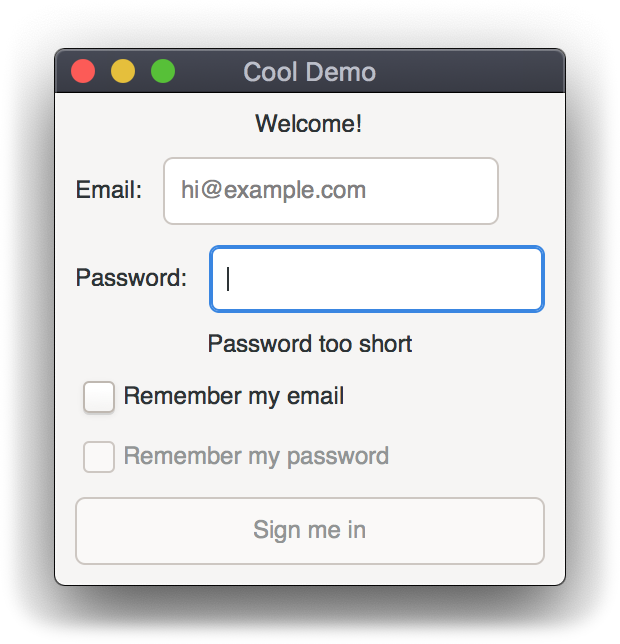
\includegraphics[width=0.4\textwidth]{loginDemo.png}
\vspace{-1.7cm}
\end{wrapfigure}

The screenshot on the right shows one of these samples, which is present in the Causson project as |samples/login.causson|. This shows a facsimile of a typical log-in screen, with fields to enter an email address and a password, and widgets that are greyed out when not relevant.

When the `Sign me in' button is clicked (which is only possible when the email address field is non-empty and the password field contains text within the accepted length bounds), the window closes and a new window appears, greeting the `user' by the email address they entered.

This example connects together multiple built-in and user-defined components by using both event handlers and dynamic properties. The error-checking makes use of the built-in string manipulation functions.

These sample programs were also extremely useful for highlighting areas where the framework was deficient. The ability to define dynamic `output' properties on components (so that they could feed data back to their parents) was left out of the language for much of the development process, but was added at a late stage during the creation of the `Goodpizza' pizza ordering example (which will be presented in the next chapter).

Similarly, \cref{secGtkCompShite} described how the `transient add' feature was added to the component system after the experimental sample programs demonstrated a need for it.

\chapter{Results and Evaluation} \label{chapResults}

This chapter will describe the current state of the Causson project, compare it to the original objectives from \cref{secHLObjectives} and requirements set out in \cref{chapSpec}, show a fully-featured sample application and discuss avenues for future improvement. Following that will be some reflection on the development process, examining where things didn't go to plan and what could have been better with more foresight.

\section{Final Prototype Overview}

The provided Causson interpreter is able to execute programs that can interact with the outside world through the GUI library and basic file access. There are various limitations that would need to be resolved before it could be used to write production-quality programs, but the current version is functional enough to serve as a vehicle for experimentation and a foundation for further improvements to be made.

The standard library is quite barebones but there are plenty of extension points for new functionality to be added - in particular, the GTK library that powers the user interface exposes lots of features which are not currently available through the Causson bindings, owing to lack of development time.

This prototype takes the form of a Rust package with roughly 4,400 lines of code, and dependencies on the following `crates' (libraries):

\begin{itemize}[nosep,topsep=0pt]
    \item \textbf{pest} (and its associated \textbf{pest-derive}), for parsing expression grammars\cite{pest}
    
    \item \textbf{lazy\_static}, for defining program-global static values using non-trivial types\cite{lazy_static}
    
    \item \textbf{symbol}, for treating IDs in the language as globally-interned strings\cite{symbol}
    
    \item \textbf{gtk} and \textbf{gio}, from \emph{gtk-rs}, for rendering GUIs using GTK\cite{gtkrs}
    
    \item \textbf{paste}, for combining strings together in Rust macros\cite{paste}
\end{itemize}

Documentation is provided in this report, with \cref{chapDesign,chapImpl} giving a narrative overview of the system, and \cref{adxGuide,adxMaint} providing a `user guide' (explaining the language from the viewpoint of a prospective user) and a `maintenance guide' (describing in further depth how to perform development tasks such as adding new built-in types).

\section{Revisiting the Requirements} \label{secReqsRetro}

The table on the following pages will go through each point on the requirements presented in \cref{secRequirements} and describe how they have been met, with a brief summary of their suitability and any significant limitations.

\begin{landscape}

\begingroup
\parindent=0cm

{\rowcolors{3}{white}{gray!08}
\begin{tabularx}{730pt} {| >{\hsize=210pt\raggedright\arraybackslash}X | >{\raggedright\arraybackslash}X |}
\hline
\hiderowcolors
    \textbf{Requirement}&\textbf{Evaluation of the outcome}\\
\showrowcolors
    \hline
    Use a familiar syntax&The syntax takes inspiration from Rust, and should be readable to programmers who are used to languages like C and Java. Blocks are delimited by curly braces and statements are ended by line breaks.\\
    \hline
    \multicolumn{2}{|l|}{\textit{Static type checking}}\\
    \hline
    Use a static type system&The entire program is type-checked before any code is executed, so errors such as mismatched types or calls to non-existent methods are detected right away (with the sole exception of \verb|Notifier|, which dispatches method calls at runtime). A limited form of type inference is available when defining local variables using \verb|let|. There are no implicit conversions between types.\\
    \hline
    Support integers and real numbers&Built-in, primitive \verb|int| (signed 64-bit integer) and \verb|real| (double-precision floating point) types are included, with all the standard comparison and arithmetic operations available.\\
    \hline
    Support tuples, records and sum types&Records and sum types (as `enum's) are fully implemented. Tuples were not included due to time constraints, since most use cases for them can also be met by records.\\
    \hline
    Built-in strings and collections&The standard library provides \verb|str|, wrapping Rust's UTF-8 strings, and \verb|List<T>|, a generic list type.\\
    \hline
    User-defined types&Programs can define new records, new enums, and single-element wrappers around other types. These can include instances of the built-in generic types, but user-defined types cannot themselves be generic. Hence, given a new record \verb|R|, creating a \verb|List<R>| is possible and adding a \verb|List| of a concrete type to \verb|R|'s fields is also possible, but \verb|R| itself cannot have a type parameter.\\
    \hline
    \multicolumn{2}{|l|}{\textit{Automatic memory management}}\\
    \hline
    Variables store references to objects&Integers, real numbers, booleans and enums are all stored by value. All other types are stored as references to objects on the heap, so assigning a variable containing a \verb|List| to another variable will create two variables that reference the same list and not two distinct lists.\\
    \hline
    Garbage collection&The skeleton for a simple garbage mark-and-sweep collector has been implemented into the interpreter, but owing to time constraints, blocks are not yet freed from memory.\\
    \hline
    \multicolumn{2}{|l|}{\textit{General programming language features}}\\
    \hline
    Stand-alone functions&Functions can be defined that accept any number of arguments and return a value. Overloading is supported, so functions can share the same name as long as they can be disambiguated through different numbers or types of arguments. Functions cannot accept variable numbers of arguments.\\
\hline
\end{tabularx}
}

{\rowcolors{3}{white}{gray!08}
\begin{tabularx}{730pt} {| >{\hsize=210pt\raggedright\arraybackslash}X | >{\raggedright\arraybackslash}X |}
\hline
\hiderowcolors
    \textbf{Requirement}&\textbf{Evaluation of the outcome}\\
\showrowcolors
    \hline
    Methods on built-in and user-defined types&Static and non-static (accepting a special `self' argument) methods can be added to any type. While user code can add methods to the built-in types, it cannot replace or shadow existing ones.\\
    \hline
    Operators implemented as methods&Binary operators such as \verb|+| and \verb|==| are mapped to method calls on the left-hand operand, allowing user code to implement operators for custom types using the same approach that is used to implement normal methods.\\
    \hline
    Control structures and loops&If-then-else structures and while loops are available and can be used in place of any expression.\\
    \hline
    Pattern matching on composite types&Enums/sum types can be accessed using the \verb|match| construct, which is the only way to extract data stored inside of one. The implementation in Causson is somewhat limited compared to that in languages such as Haskell, as it simply unpacks the values into local variables but does not perform any comparisons on them or allow for recursive matching.\\
    \hline
    Error handling through sum types&Implemented to a limited extent: the \verb|io:File| type used for accessing files uses the built-in \verb|Maybe<T>| type for return values to distinguish between success and failure.\\
    \hline
    \multicolumn{2}{|l|}{\textit{Component system}}\\
    \hline
    Can be used to represent concepts other than GUIs&The component system is not tied directly to the GUI types. Any types that conform to a specific interface (e.g. including the \verb|add_child| method) may be used with it.\\
    \hline
    Properties storing arbitrary data&Two forms of properties are allowed inside components: simple fields that can be read and written to, and dynamic properties which are computed expressions that get automatically updated.\\
    \hline
    Methods containing code&Methods can be included which are available directly on the component type.\\
    \hline
    Emits events/signals for other components&Partially implemented; built-in types like \verb|gui:Button| define signals which can be connected to. There is currently no specific syntax for user-defined components to define their own signals, but the same behaviour can be simulated by creating a property and writing to it to trigger the signal.\\
    \hline
    Declaratively specifies sub-components&Components can include hierarchies of any depth by using the special \verb|add_child| method and \verb|root| property. User-defined components can be nested inside each other.\\
    \hline
    Declaratively specifies data dependencies between properties&Property assignments are scanned to determine what values they access so that they can be updated automatically when those values change, without requiring the programmer to write explicit synchronisation code. This works with some limitations; cycles are not detected, some built-in properties cannot be dependencies, and the scanner will not look inside methods defined outwith the component it's scanning.\\
\hline
\end{tabularx}
}

{\rowcolors{3}{white}{gray!08}
\begin{tabularx}{730pt} {| >{\hsize=210pt\raggedright\arraybackslash}X | >{\raggedright\arraybackslash}X |}
\hline
\hiderowcolors
    \textbf{Requirement}&\textbf{Evaluation of the outcome}\\
\showrowcolors
    \hline
    Declaratively specifies connections between signals and code&Blocks of code and calls to existing methods can be attached to signals.\\
    \hline
    \multicolumn{2}{|l|}{\textit{Built-in APIs}}\\
    \hline
    String manipulation&Simple operations are provided to concatenate strings, check their length, and convert numbers to strings.\\
    \hline
    Data structures and collections&A generic \verb|List<T>| type is provided which holds any number of elements, backed by Rust's \verb|Vec| type. Lists may be contain any type, including user-defined types.\\
    \hline
    File input/output&Text files can be read and written by using the methods provided on the \verb|io:File| type.\\
    \hline
    Graphical user interfaces&The types and functions inside the \verb|gui| namespace wrap a subset of the GTK library, offering the creation of windows, nestable horizontal/vertical layouts, push buttons, check boxes, radio buttons, single-line text fields, drop-down boxes, text labels, images, tabbed areas and bordered/framed boxes.\\
    \hline
    Networking (if time allowed)&This was omitted to focus on enhancing other aspects.\\
    \hline
    \multicolumn{2}{|l|}{\textit{Quality-of-Life Features}}\\
    \hline
    Documentation&This report includes a `user guide' (manual for the language) in its appendices.\\
    \hline
    Error reporting&The pre-execution phases of the Causson interpreter will generate reports if an error is detected, but there is significant room for improvement in this area. Syntax errors will flag up the relevant position in the source code, but errors in later phases do not use this information and only show a description and some minimal state related to the error.\\
\hline
\end{tabularx}
}

\endgroup

\end{landscape}

\section{Sample Application: `Goodpizza'}

The main sample application developed in Causson is a hypothetical pizza ordering interface, present inside the distribution at |samples/pizza.causson|.

It demonstrates almost every feature in the language: defining new types, defining components and composing them together, building a GUI with a nested layout, manipulating numbers and strings, and writing files.

Each `step' shown in the interface - selecting a pizza size, a sauce, and toppings - is handled by a stand-alone component and has zero knowledge about the other steps. The window shows a total price which is kept up-to-date through the property mechanism in Causson's components system, and when complete, the user can click the `Generate Order' button which fetches the information from the three components and writes it to a file.

\begin{Verbatim}
gui:Frame {
    .label = Maybe<str>:Just("Step 1: Pick a size")
    size = PizzaSizeChooser
}

gui:Frame {
    .label = Maybe<str>:Just("Step 2: Pick a sauce")
    sauce = PizzaSauceChooser
}

gui:Frame {
    .label = Maybe<str>:Just("Step 3: Pick toppings")
    toppings = ToppingsChooser {
        .toppingPrice = self.size.toppingSurcharge
        .includedToppings = self.size.includedToppings
    }
}

gui:Label {
    .markup = "Your total is " + formatPrice(self.total())
}
\end{Verbatim}

Consider the above fragment, extracted from the |PizzaForm| component in the Goodpizza application. Note how the total label has its text defined using an expression that contains |self.total()|. The Causson interpreter looks inside the definition for the |total| method and sees references to the three |price| properties, so these are considered to be dependencies. Hence, whenever those |price| properties change, the total label is automatically updated.

As a result, there is no need to write explicit synchronisation code that updates the total. The code is more expressive, as the single |gui:Label| block shown above tells a reader everything about the label. Its location in the resulting UI is based off where in the hierarchy it appears. It doesn't even need to have a name, as it's a simple output and there is no reason to reference it from other code.

In contrast, consider how this scenario would be implemented using the |JLabel| class in Java's Swing framework. A field would need to be added in the class scope to store the label. The label object needs to be created and then added into the layout at an appropriate location. This involves three separate pieces of code, in different locations, just for a label with static text.

In order to keep it up-to-date, a method would have to be written that calculates the new total and updates the label's text. This method would then need to be connected to the three `step' components (as they all influence the total price), typically by implementing either the Listener pattern or the Observer pattern.

\subsection{Architectural Diagram}

The following page shows a screenshot of the Goodpizza interface and a diagram of the components involved that shows how data flows within the interface to keep the price displays up-to-date when the user interacts with elements.

\begingroup
\parindent=0cm
For readability, the diagram omits some elements:
\endgroup

\begin{itemize}[nosep,topsep=0pt]
    \item The `Welcome to Goodpizza' title label (as it is purely visual)
    
    \item The `Big Toste` animated pizza graphic (rendered using a |gui:Image| component)
    
    \item The nested vertical/horizontal boxes that lay out the user interface
    
    \item The methods returning |PizzaSize|, |PizzaSauce| and |List<Topping>| values that the three step components provide (which are used when the `Generate Order' button is clicked)
\end{itemize}

\subsection{Maintaining the App}

Consider a hypothetical scenario where Goodpizza decides to expand their business and begin offering calzones and pasta dishes, so they need to update their ordering app. They first create the new components |CalzoneForm| and |PastaForm|, and then update the |GoodpizzaApp| component so that the three forms are presented inside tabs using |gui:Notebook|.

The |PizzaForm| remains unchanged. Since it just returns a |gui:Widget| as its root, this slots into the notebook the same way that it did when it was added into a box before.

Goodpizza's chef is conscious about food waste and has decided that they will offer the same topping options on their new dishes as they do on their pizzas, rather than ordering different supplies. As a result, the |ToppingsChooser| component can be re-used with no changes.

They also decide to re-use the |PizzaSauceChooser| for calzones, as they will be offering the same three options even though the base price and sizes are different from those used for pizzas.

The nature of the component system in Causson makes it very straightforward to implement separate blocks of functionality in fully decoupled components, and this pays off when changes like this are required.

\vspace{1mm}

%\hspace*{-1.5cm}\vspace*{-1.5cm}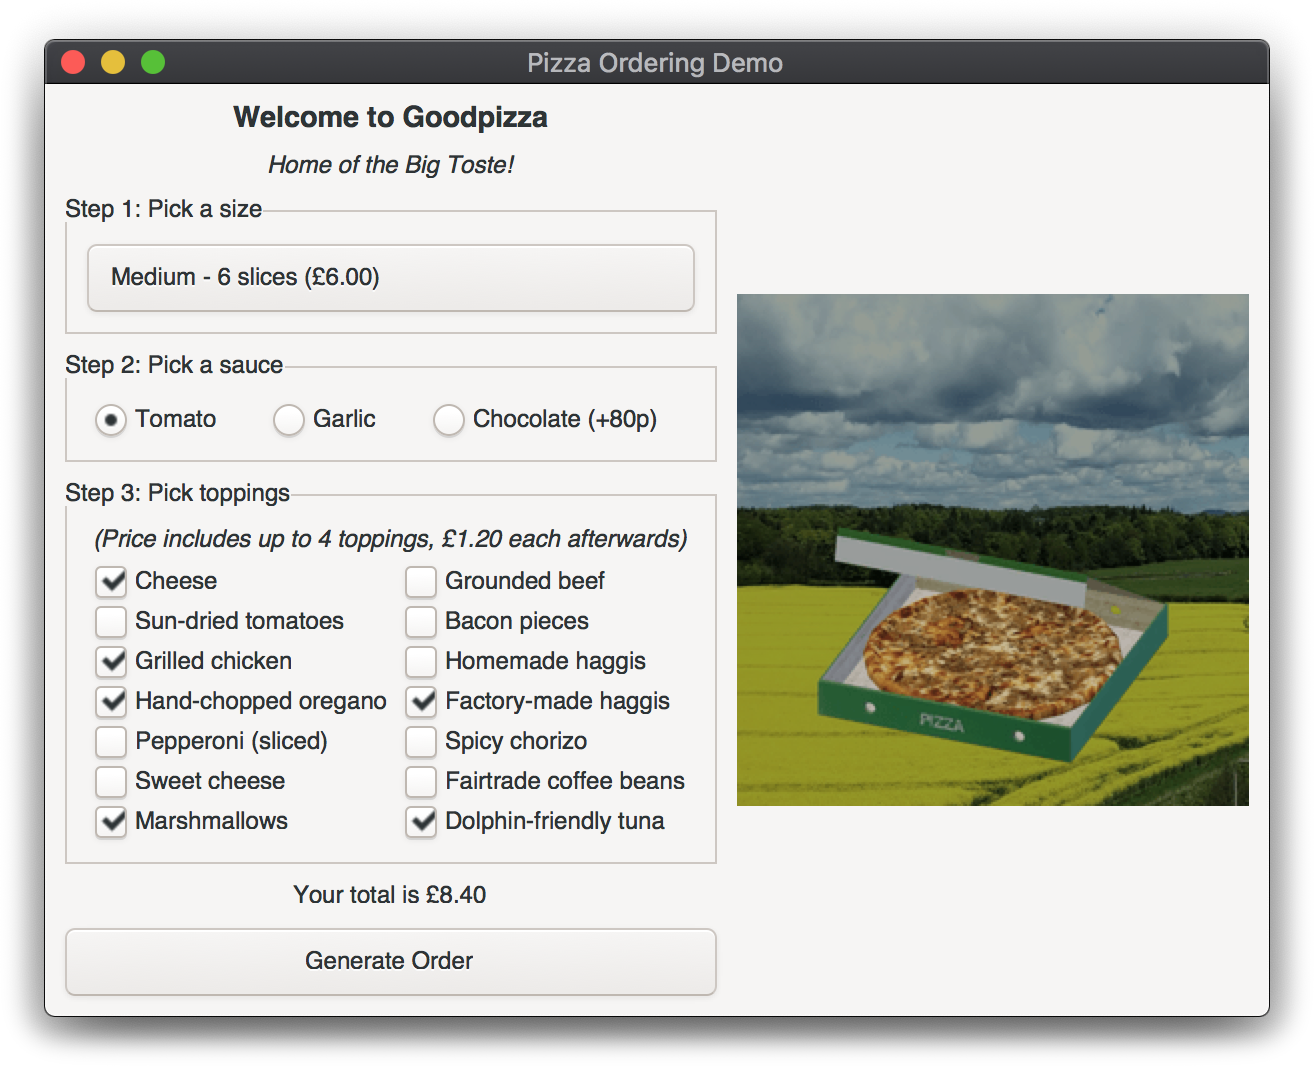
\includegraphics[width=1.1\textwidth]{goodpizza.png}
\vspace*{-1.5cm}\hspace*{-1.5cm}\begin{tikzpicture}[
cblip/.style={circle, draw=black!60, fill=red!5, very thick, minimum size=5mm, execute at begin node=C, drop shadow},
expl/.style={rectangle, draw=black!60, fill=white!90, very thick, anchor=east, rounded corners, drop shadow, inner sep=6.0},
arrow/.style={->, draw=blue!60, very thick},
holder/.style={draw=blue!60, very thick},
holderL/.style={draw=red!40!black, very thick}
]
\node {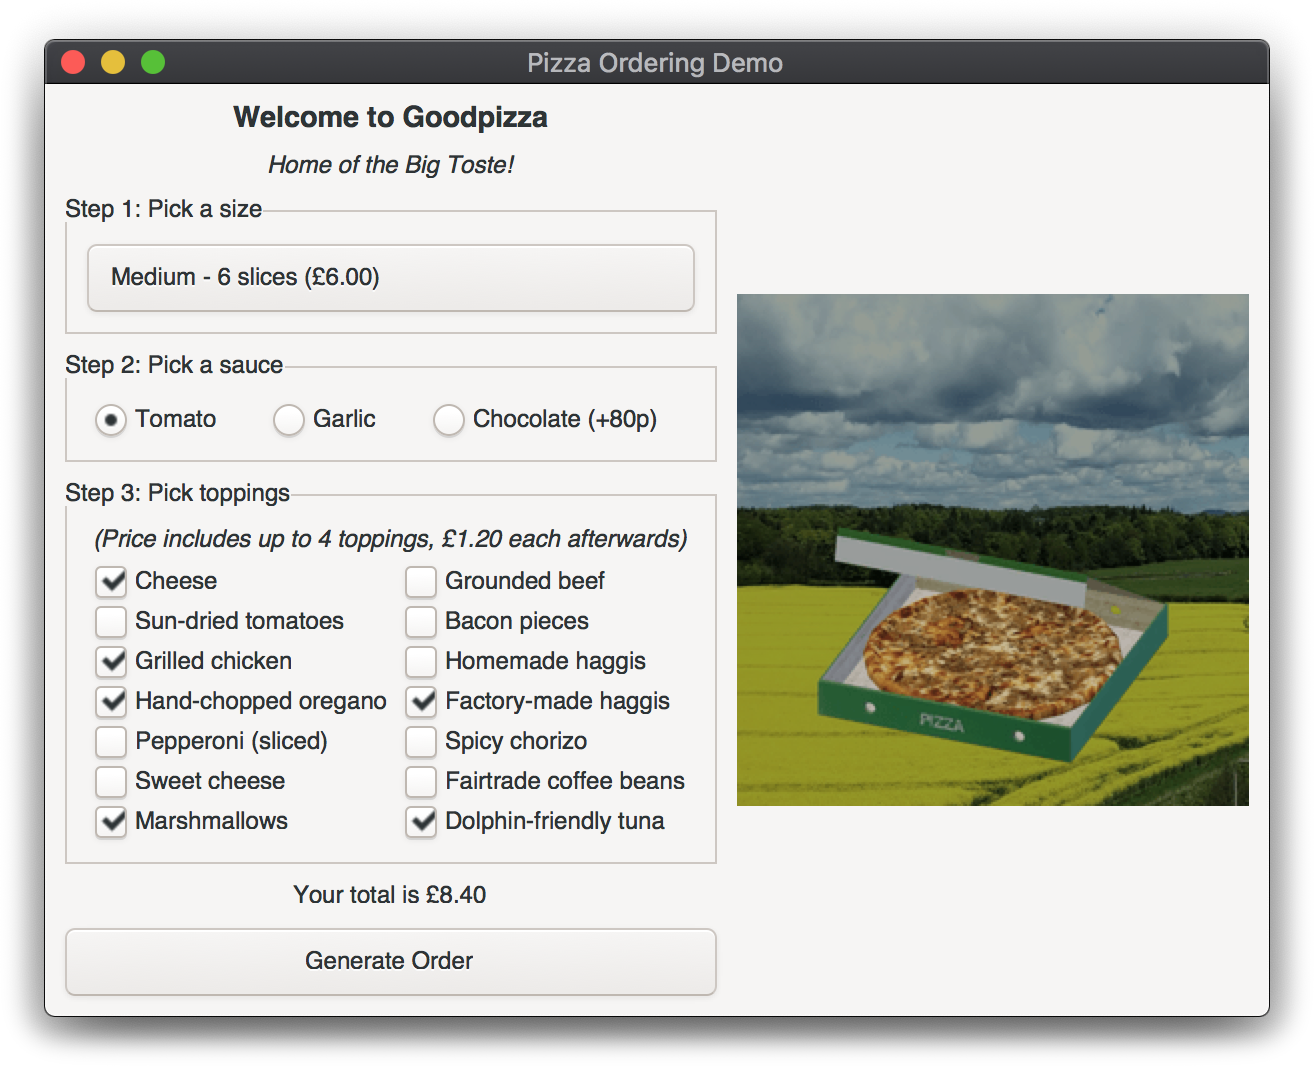
\includegraphics[width=1.1\textwidth]{goodpizza.png}};
%\node[cblip] at (4,6.5) {0};
%\draw[holderL] (-8.5,3.5) -- ++(0,3);
%\draw[holderL] (-8.5,3.5) -- ++(0,-3);
\node[cblip] at (-8.5,3.5) {1};
\node[cblip] at (-8.5,1.65) {2};
\node[cblip] at (-8.5,-2.0) {3};

\node[expl, text width=6.0cm] at (8.0,3.5) (size) {pizza is selected using a drop-down box, the |gui:ComboBoxText| widget};
\node[expl, text width=4.7cm] at (8.0,1.6) (sauce) {sauce is selected using three |gui:RadioButton| widgets};
\node[expl, text width=6.2cm] at (8.0,-0.1) (tprice) {displays the topping prices passed in through the inputs, using |gui:Label|};
\node[expl, text width=6.1cm] at (8.0,-2.3) (tcheck) {14 |gui:CheckButton| widgets allow toppings to be turned on and off};
\node[expl, text width=6.5cm] at (8.0,-4.0) (total) {displays the total price using |gui:Label|};
\node[expl, text width=5.0cm] at (8.0,-5.9) (butt) {order is written to a file when this |gui:Button| is clicked};
\draw[arrow] (size.west) -- (0.52,3.5);
\draw[holder] (sauce.west) -- (0.3,1.6);
\draw[holder] (0.3,1.6) -- ++(0,0.3) -- ++(-0.2,0);
\draw[holder] (0.3,1.6) -- ++(0,-0.3) -- ++(-0.2,0);
\draw[arrow] (tprice.west) -- (0.5,-0.1);
\draw[holder] (tcheck.west) -- (0.6,-2.3);
\draw[holder] (0.6,-2.3) -- ++(0,1.9) -- ++(-0.2,0);
\draw[holder] (0.6,-2.3) -- ++(0,-1.9) -- ++(-0.2,0);
\draw[arrow] ($(total.south west) + (1.5,0)$) |- (-2.2,-5.0);
\draw[arrow] (butt.west) -- (0.8,-5.9);

%\node[expl, text width=6.0cm] at (0.9,3.5) {Pizza is selected using a drop-down box, the |gui:ComboBoxText| widget};
%\node[expl, text width=4.7cm] at (0.9,1.65) {Sauce is selected using three |gui:RadioButton| widgets};
%\node[expl, text width=6.2cm] at (0.9,-0.1) {displays the topping prices passed in through the inputs, using |gui:Label|};
%\node[expl, text width=6.1cm] at (0.9,-2.0) {14 |gui:CheckButton| widgets allow toppings to be turned on and off};
%\node[expl, text width=6.5cm] at (0.9,-5.0) {displays the total price using |gui:Label|};
%\node[expl, text width=5.0cm] at (0.9,-6.0) {order is written to a file when this |gui:Button| is clicked};
%\draw[arrow] (0.9,-6.0) -- (0.6,-6.0);
\end{tikzpicture}


\vspace*{-0.5cm}\hspace*{-0.8cm}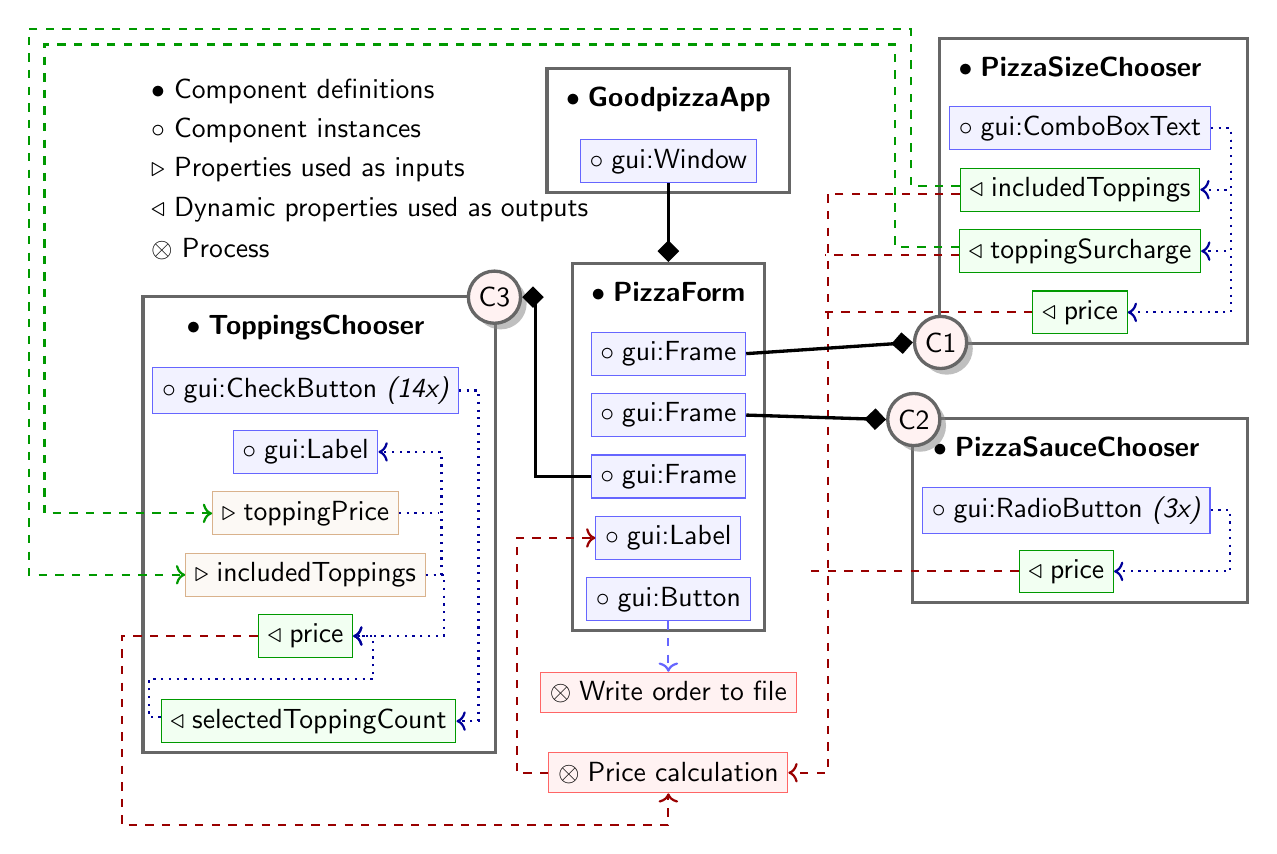
\begin{tikzpicture}[
cblip/.style={circle, draw=black!60, fill=red!5, very thick, minimum size=5mm, execute at begin node=C, drop shadow, inner sep=2},
comp/.style={rectangle, draw=black!60, very thick, minimum size=5mm},
title/.style={anchor=west, font=\bf, execute at begin node=$\bullet$\hspace{0.1cm}},
instbox/.style={rectangle, draw=blue!60, fill=blue!2, anchor=west},
instboxt/.style={anchor=west, execute at begin node=$\bullet$\hspace{0.1cm}},
inst/.style={rectangle, draw=blue!60, fill=blue!5, anchor=west, execute at begin node=$\circ$\hspace{0.1cm}},
oprop/.style={rectangle, draw=green!60!black, fill=green!5, anchor=west, execute at begin node=$\triangleleft$\hspace{0.1cm}},
iprop/.style={rectangle, draw=brown!60, fill=brown!5, anchor=west, execute at begin node=$\triangleright$\hspace{0.1cm}},
func/.style={rectangle, draw=red!60, fill=red!5, anchor=west, execute at begin node=$\otimes$\hspace{0.1cm}},
arrow/.style={-Turned Square, very thick},
dataArrow/.style={->, dashed, thick, draw=green!60!black},
priceArrow/.style={->, dashed, thick, draw=red!60!black},
priceArrowN/.style={dashed, thick, draw=red!60!black},
intdataArrow/.style={->, dotted, thick, draw=blue!60!black},
intdataArrowN/.style={dotted, thick, draw=blue!60!black},
actionArrow/.style={->, dashed, thick, draw=blue!60},
]

%\begin{scope}[on background layer]
%\end{scope}

\node[title] (wndTitle) {GoodpizzaApp};
\node[inst, below=0.5cm of wndTitle.center] (wndWnd) {gui:Window};
\begin{scope}[on background layer]
    \node[comp, fit={(wndTitle) (wndWnd)}] (wnd) {};
\end{scope}

\node[title, below=1cm of wnd.south] (pzTitle) {PizzaForm};
\node[inst, below=0.5cm of pzTitle.center] (pzFrame1) {gui:Frame};
\node[inst, below=0.5cm of pzFrame1.center] (pzFrame2) {gui:Frame};
\node[inst, below=0.5cm of pzFrame2.center] (pzFrame3) {gui:Frame};
\node[inst, below=0.5cm of pzFrame3.center] (pzLabel) {gui:Label};
\node[inst, below=0.5cm of pzLabel.center] (pzButton) {gui:Button};
\node[comp, fit={(pzTitle) (pzFrame1) (pzFrame2) (pzFrame3) (pzLabel) (pzButton)}] (pizza) {};

\node[title, right=2cm of pizza.east] (sauTitle) {PizzaSauceChooser};
\node[inst, below=0.5cm of sauTitle.center] (sauRadios) {gui:RadioButton \emph{(3x)}};
\node[oprop, below=0.5cm of sauRadios.center] (sauOut1) {price};
\node[right=0.1cm of sauRadios.east] (sauDummy) {};
\node[comp, fit={(sauTitle) (sauRadios) (sauOut1) (sauDummy)}] (sauce) {};
\draw[intdataArrow] (sauRadios.east) -- ++(0.25,0) |- (sauOut1.east);

\node[title, above=4.2cm of sauce.north] (szTitle) {PizzaSizeChooser};
\node[inst, below=0.5cm of szTitle.center] (szCombo) {gui:ComboBoxText};
\node[oprop, below=0.5cm of szCombo.center] (szOut1) {includedToppings};
\node[right=0.1cm of szCombo.east] (szDummy) {};
\node[oprop, below=0.5cm of szOut1.center] (szOut2) {toppingSurcharge};
\node[oprop, below=0.5cm of szOut2.center] (szOut3) {price};
\node[comp, fit={(szTitle) (szCombo) (szOut1) (szOut2) (szOut3) (szDummy)}] (size) {};
\draw[intdataArrow] (szCombo.east) -- ++(0.25,0) |- (szOut1.east);
\draw[intdataArrow] (szCombo.east) -- ++(0.25,0) |- (szOut2.east);
\draw[intdataArrow] (szCombo.east) -- ++(0.25,0) |- (szOut3.east);

\node[title, below left=2cm of wnd.south west] (topTitle) {ToppingsChooser};
\node[inst, below=0.5cm of topTitle.center] (topChecks) {gui:CheckButton \emph{(14x)}};
\node[right=0.1cm of topChecks.east] (topDummy) {};
\node[inst, below=0.5cm of topChecks.center] (topLabel) {gui:Label};
\node[iprop, below=0.5cm of topLabel.center] (topIn1) {toppingPrice};
\node[iprop, below=0.5cm of topIn1.center] (topIn2) {includedToppings};
\node[oprop, below=0.5cm of topIn2.center] (topOut1) {price};
\node[oprop, below=0.8cm of topOut1.center, xshift=1.1] (topOut2) {selectedToppingCount};
\draw[intdataArrowN] (topIn1.east) -- ++(0.5cm,0);
\draw[intdataArrow] (topIn2.east) -| ($(topLabel.east) + (0.8cm,0)$) -- (topLabel.east);
\draw[intdataArrow] ($(topOut2.west) + (0,0.05cm)$) -| ($(topOut2.north west) + (-0.15cm,0.25cm)$) -| ($(topOut1.east) + (0.25cm,0)$) -- (topOut1.east);
\draw[intdataArrow] (topIn2.east) -| ($(topOut1.east) + (1.15cm,0)$) -- (topOut1.east);
\draw[intdataArrow] (topChecks.east) -- ++(0.25cm,0) |- (topOut2.east);

\node[comp, fit={(topTitle) (topLabel) (topChecks) (topIn1) (topIn2) (topOut1) (topOut2) (topDummy)}] (toppings) {};

\node[func, below=0.5cm of pizza.south] (fnOrder) {Write order to file};
\node[func, below=0.5cm of fnOrder.south] (fnPrice) {Price calculation};

\draw[dataArrow] ($(szOut1.west) + (0,0.05cm)$) -| (4.5,0.9) -- (-6.7,0.9) |- (topIn2.west);
\draw[dataArrow] ($(szOut2.west) + (0,0.05cm)$) -| (4.3,0.7) -- (-6.5,0.7) |- (topIn1.west);

\draw[priceArrow] ($(szOut1.west) - (0,0.05cm)$) -| ($(fnPrice.east) + (0.5cm,0)$) -- (fnPrice.east);
\draw[priceArrowN] ($(szOut2.west) - (0,0.05cm)$) -- ++(-1.7cm,0);
\draw[priceArrowN] (szOut3.west) -- ++(-2.7cm,0);
\draw[priceArrowN] (sauOut1.west) -- ++(-2.7cm,0);
\draw[priceArrow] (topOut1.west) -| ($(toppings.south west) - (0.25cm,0.9cm)$) -| (fnPrice.south);
%\draw[priceArrowN] ($(topOut2.west) - (0,0.05cm)$) -- ++(-0.55cm,0);
\draw[priceArrow] (fnPrice.west) -| ($(pzLabel.west) - (1.0cm,0)$) -- (pzLabel.west);

\draw[actionArrow] (pzButton.south) -- (fnOrder.north);

\node[above=5.5cm of toppings.west, anchor=west] (key1) {$\bullet$ Component definitions};
\node[below=0.5cm of key1.west, anchor=west] (key2) {$\circ$ Component instances};
\node[below=0.5cm of key2.west, anchor=west] (key3) {$\triangleright$ Properties used as inputs};
\node[below=0.5cm of key3.west, anchor=west] (key4) {$\triangleleft$ Dynamic properties used as outputs};
\node[below=0.5cm of key4.west, anchor=west] (key5) {$\otimes$ Process};

\node[below left=-0.4cm of size, cblip] (blip1) {1};
\node[above left=-0.4cm of sauce, cblip] (blip2) {2};
\node[above right=-0.4cm of toppings, cblip] (blip3) {3};

\draw[arrow] (wndWnd.south) -- (pizza.north);
\draw[arrow] (pzFrame1.east) -- (blip1.west);
\draw[arrow] (pzFrame2.east) -- (blip2.west);
%\draw[arrow] (pzFrame3.west) -- ++(-1.6,0);
\draw[arrow] (pzFrame3.west) -- ++(-0.7,0) |- (blip3.east);

\end{tikzpicture}

\section{Future Improvements to Causson}

There is significant room for expansion to the language in order to allow for more practical applications to be written in it. Some of these involve fixing limitations that were identified in \cref{secReqsRetro} (\emph{\nameref{secReqsRetro}}), while others involve potential additions that were not covered in the original objectives at all.

\subsection{Additions to Typing}

The type system in Causson is extremely simple and does not allow for dynamic dispatch of method calls with the key exception of the |Notifier| object, a kludge that works around this in a way that cannot be checked before the code executes.

There are different approaches that could have been taken to make this work, but all of them would have added significant complexity to the project.

The language would benefit from the ability to determine when types can be converted in a non-ambiguous way. Currently, if a property accepts a |Maybe<str>| (such as the label on |gui:Frame| widgets), you cannot assign a string directly and must instead obtain the appropriate value by calling into the fully qualified name \fbox{\Verb/Maybe<str>:Just(...)/}.

Since property setters are just methods, and methods can be overloaded, this could in theory be implemented on a property-by-property basis by providing both |label=(Maybe<str>)| and |label=(str)| methods.

It would however be cleaner if the interpreter could detect that there is only one possible target type and automatically convert the string to the target type. Another way to improve this would be by allowing enum choices (like |Just(...)|) to be used in expressions without having to qualify them with the full type name.

Additionally, the current system for generic types does not allow generic code to be written in Causson itself as the type checker requires concrete types and there is no facility to defer this checking to a later stage. Hence, there is no way for user code to implement its own version of a built-in type like |Maybe<T>|.

\subsection{Language Constructs}

Inside functions, methods and other locations that accept expressions, programs have access to basic \emph{if-then-else} structures and \emph{while} loops. The current implementations work, but could be expanded.

There is no support for the usual |break| and |continue| keywords inside loops, so implementing these would be an obvious step forward. The ability to iterate over ranges and containers using \emph{for-each} loops would also be good. This is still possible using the existing features, but not as elegant.

A very basic form of pattern-matching is provided which simply operates on enums, by using the value of the enum to determine which sub-expression to evaluate, and unpacking the data it holds into local variables. This is the bare minimum needed to work with enums, but it would be much more interesting if patterns were also able to match data and recurse into sub-structures as is possible in other languages.

\subsection{Interpreter Features}

The garbage collector in the interpreter is partially implemented but not fully functional, so fixing that would be one of the highest priorities for future development of the project. For the purposes of experimenting with language features, it's not necessary, but real-world software written in Causson would not be able to get away with leaking memory continuously\footnote{Many commercial software products do this, but that doesn't make it a good thing.}.

There has also been no work done to optimise the interpreter. Speed has not been an issue for the test programs written so far, but it could pose a problem for more involved tasks.

\subsection{Components}

The current version of the component system is promising, but very much a prototype. The approach used to implement it by generating code makes it unable to detect certain kinds of mistakes, which result in confusing error messages when later phases of the processing attempt to type-check the generated code.

Not all properties implement the notifier system, so dynamic properties depending on these will not update correctly. There are certain constructs which will not be scanned correctly by the algorithm that checks for dependencies.

For scenarios where widgets need to be added or removed dynamically (such as an editor with multiple files in different tabs), the declarative approach used in Causson's components does not help. A solution to this would be a very interesting improvement, but it would also require significant architectural changes to the component system.

\subsection{Standard Library}

There are many features missing from the standard library which would be necessary for more practical code, which have been omitted from this prototype in the interests of dedicating development time towards solving more interesting problems. The following list presents some ideas.

\begin{itemize}
    \item \textbf{Core Types}
    
    \begin{itemize}[nosep,topsep=0pt]
        \item Bitwise operations on integers
        
        \item Common mathematical operations for real numbers (square root, raising to a power, trigonometric functions, etc.)
        
        \item Extracting characters and substrings from strings
        
        \item Unsigned integers
        
        \item A byte array or buffer type, for working with binary data
    \end{itemize}

    \item \textbf{Data Structures}
    
    \begin{itemize}[nosep,topsep=0pt]
        \item More utility methods for |List<T>|
        
        \item A |Map<K,V>| type using the existing infrastructure for generic types
    \end{itemize}
    
    \item \textbf{Operating System and Utility Features}
    
    \begin{itemize}[nosep,topsep=0pt]
        \item Extending |io:File| to work with binary data, allow seeking, and partial reads
        
        \item Adding more |io| features to operate on files and directories
        
        \item Facilities to call into other processes, get environment variables and arguments, and read standard input

        \item Functions for working with times and dates
        
        \item Random number generation
    \end{itemize}
    
    \item \textbf{User Interfaces}

    \begin{itemize}[nosep,topsep=0pt]
        \item Binding to more GTK features: grid layouts, menus, multi-line text views, open/save dialog boxes, etc.
        
        \item Exposing all of the options offered by the widgets that are available
        
        \item Access to the graphic drawing features offered by GTK through the underlying Cairo library
    \end{itemize}
\end{itemize}

\subsection{Error Handling}

One of the goals for this project was to use sum types for representing situations such as errors. The prototype implements this to an extent, and the core language provides the required infrastructure, but there is room for improvement.

With the limited functionality present in the standard library, the only actions that can currently raise errors are file input/output. These are handled by returning a |Maybe<T>| from operations that can fail, where |None| represents a failure. Ideally, this would use a type that actually encodes information about what the error was.

\section{Development Process}

Finally, this section aims to evaluate the processes involved in building this project and how they affected the final product.

The original brief for this project was extremely open-ended on purpose - `build a programming language'. As discussed in \cref{chapSpec,chapDesign} (\emph{\nameref{chapSpec}, \nameref{chapDesign}}), the process began with various experiments using both Haskell and Rust, aiming to pin down what was feasible in the hopes of making it easier to decide on a niche.

In some ways, the amount of possibilities available were both a blessing and a curse. It would have been easy to build something straightforward like an implementation of BASIC, a language so simple that it was built into computers from the 1980s, but this felt like a bit of a cop-out.

There was also a very real risk that the goals would end up being set too high and the project would be too difficult to complete within the available timeframe - which did end up happening in the end, to an extent.

The decision to build an imperative language with a focus on GUIs was an attempt to strike a balance between these two, by building something fairly traditional but also trying to innovate at the same time.

Choosing Rust as an implementation language was also an uncertain bet. Although Rust has many resources behind it, it is fairly new compared to languages such as C++ and Python. Its safety guarantees are one of its biggest selling points, but they also make it very difficult to write code at times.

The early development of Causson was very slow because frustration caused by battling with Rust's borrow checker led to the project frequently being put aside.

Rewriting it in another language was considered, but this would have meant dropping the existing progress and having to find new libraries for parsing. It would also have meant losing out on the advantages of Rust, such as first-class sum types, which proved to be extremely enjoyable to use even in spite of the issues incurred by the borrow checker.

With time and more experience it became easier to write Rust code, and the project developed at a much faster rate once the foundation was in place.

It's difficult to say whether the result would have been better or worse if it had been implemented in a different language. It would certainly have been easier to deal with memory management in a language that didn't enforce Rust's safety guarantees, but that would of course also come with a higher risk of bugs.

\section{Conclusion}

The Causson project has produced a language specification and a prototype interpreter which is able to execute a variety of programs.

From the beginning of development, the Causson project was viewed as experimental, with the understanding that some of the decisions made might not end up being optimal and that there simply would not be enough time to build it out into a full, production-quality product.

With this point of view, the project appears to be fairly successful. There are various limitations and aspects which didn't quite work out, but the result meets almost all of the requirements set out at the beginning, as well as including some features which weren't in the original plans.



\clearpage
\appendix
\titleformat
{\chapter} % command
[display] % shape
{\vspace{.8ex}\normalfont\large\itshape} % format
{\filright Appendix \thechapter\enspace} % label
{0.2ex} % sep
{\titlerule
\vspace{.2ex}\Huge%
} % before-code
[\vspace{.2ex}%
\titlerule] % after-code
\pagestyle{appendix}

\chapter{\label{chap:Comparing-Prior-GUI}Comparing Prior GUI Systems}

This appendix expands on the research presented in \cref{secGUI}
by showing code samples for some of the frameworks discussed in that
section.

A simple example will be constructed where a counter window is created
that contains a label and three buttons (Up, Down and Zero). This
has been implemented in multiple frameworks in order to demonstrate
the approaches they take for creating an interface, connecting code
to events and updating visible attributes of the widgets.

\section{\label{sec:Appendix-Qt-Widgets}Qt Widgets}

\begin{figure}[h]
\begin{minipage}[t]{1\columnwidth - 2\fboxsep - 7.5\fboxrule - 1pt}%
\begin{minted}{c++}
class CoolWindow : public QWidget {
    Q_OBJECT

    int m_counter;
    QLabel *m_label;
    QPushButton *m_upButton, *m_downButton, *m_zeroButton;

private slots:
    void upButtonPushed();
    void downButtonPushed();
    void syncState();

public:
    CoolWindow(QWidget *parent = nullptr);
    ~CoolWindow() { }
};
\end{minted}
%
\end{minipage}\smallskip{}

\begin{minipage}[t]{1\columnwidth - 2\fboxsep - 7.5\fboxrule - 1pt}%
\begin{minted}{c++}
CoolWindow::CoolWindow(QWidget *parent) : QWidget(parent), m_counter(0) {
    setWindowTitle("Counter");

    m_label = new QLabel("0", this);
    m_upButton   = new QPushButton("Up", this);
    m_downButton = new QPushButton("Down", this);
    m_zeroButton = new QPushButton("Zero", this);

    connect(m_upButton,   &QPushButton::clicked,
            this,         &CoolWindow::upButtonPushed);
    connect(m_downButton, &QPushButton::clicked,
            this,         &CoolWindow::downButtonPushed);

    connect(m_zeroButton, &QPushButton::clicked, [this]() {
        m_counter = 0;
        syncState();
    });

    auto subLayout = new QHBoxLayout;
    subLayout->addWidget(m_upButton);
    subLayout->addWidget(m_downButton);
    subLayout->addWidget(m_zeroButton);

    auto layout = new QVBoxLayout(this);
    layout->addWidget(m_label);
    layout->addLayout(subLayout);

    syncState();
}

void CoolWindow::upButtonPushed() {
    ++m_counter;
    syncState();
}

void CoolWindow::downButtonPushed() {
    --m_counter;
    syncState();
}

void CoolWindow::syncState() {
    m_label->setText(QString::number(m_counter));
    m_upButton->setEnabled(m_counter < 10);
    m_downButton->setEnabled(m_counter > 0);
    m_zeroButton->setEnabled(m_counter != 0);
}
\end{minted}
%
\end{minipage}\caption{\label{fig:QtCounter}Counter sample in Qt Widgets C++}
\end{figure}

\Cref{fig:QtCounter} creates a window containing the appropriate elements,
and puts them into a pair of box layouts.

This example draws attention to some of the flaws inherent to the
Qt approach. The constructor is responsible for initialising model
properties (\Verb{m\_counter}), creating the widgets, connecting handlers
to them and then creating the layout.

Signal handlers can be connected to slots that are defined as class
methods (as this example does for the Up and Down buttons) or to C++
lambda functions (as this example does for the Zero button).

The former approach is full of redundancy. In order to attach code
to the button, a prototype needs to be added to the header file, the
method itself needs to be added to the implementation file, and a
call to \Verb{QObject::connect} needs to be added to the constructor.
This spreads the code for one action out into multiple places.

Using lambda functions keeps the code more concise and avoids having
to modify the header file, but the cluttered C++ syntax makes it hard
to follow, and even with this approach, the connection must be kept
separate from the code that creates the button.

The other flaw visible here is that each piece of code that modifies
the counter property must make sure it calls the \Verb{syncState}
method. In this example it's plainly visible, but in more complex
systems it can be easy to accidentally forget to request an update.

Finally, the widget layouts have to be created through a series of
method calls, so there is no obvious mapping between the visual layout
to the code. This is different to the declarative frameworks examined
in this appendix, where the definition of a widget is nested inside
the definition of its container.

\section{\label{sec:Appendix-Qt-Quick/QML}Qt Quick/QML}

\begin{figure}
\begin{minipage}[t]{1\columnwidth - 2\fboxsep - 7.5\fboxrule - 1pt}%
\begin{minted}{tex}
Window {
    visible: true
    property int counter: 0

    ColumnLayout {
        Label {
            text: counter.toString()
        }
        RowLayout {
            Button {
                text: "Up"
                enabled: counter < 10
                onClicked: counter += 1
            }
            Button {
                text: "Down"
                enabled: counter > 0
                onClicked: counter -= 1
            }
            Button {
                text: "Zero"
                enabled: counter != 0
                onClicked: counter = 0
            }
        }
    }
} 
\end{minted}
%
\end{minipage}\caption{\label{fig:QML}Counter sample in QML}
\end{figure}

\Cref{fig:QML} shows how the same example can be implemented in QML
with significantly less boilerplate code. Each button is defined inside
of the layout that contains it, so the structure of the file corresponds
to the structure of the UI itself.

The logic for each widget is self-contained within its \Verb{Label}
or \Verb{Button} block, so everything that the widget does is visible
at once. No explicit updates are necessary as the runtime knows that
the label's text and the buttons' enabled attributes depend on the
\Verb{counter} property, so whenever the property changes, those attributes
are re-evaluated.

\section{\label{sec:Appendix-SwiftUI}SwiftUI}

\begin{figure}[h]
\begin{minipage}[t]{1\columnwidth - 2\fboxsep - 7.5\fboxrule - 1pt}%
\begin{minted}{tex}
struct CoolWindow: View {
    @State var counter: Int = 0
    
    var body: some View {
        VStack {
            Text(String(counter))

            HStack {
                Button("Up", action: {
                    self.counter += 1
                }).disabled(counter >= 10)

                Button("Down", action: {
                    self.counter -= 1
                }).disabled(counter <= 0)

                Button("Zero", action: {
                    self.counter = 0
                }).disabled(counter == 0)
            }
        }
    }
}
\end{minted}
%
\end{minipage}\caption{\label{fig:SwiftUI}Counter sample in SwiftUI}
\end{figure}
The basic structure of the example in \cref{fig:SwiftUI} is quite similar
to the QML example. The window contains a \Verb{counter} property
which is initialised to zero. The UI hierarchy is built by nesting
definitions inside other definitions. No explicit updates are necessary
as the runtime automatically detects when they are required.

The UI syntax is not quite as consistent or elegant as QML,
owing to the fact that it's implemented using Swift metaprogramming
and has to abide by its rules. In this example, we specify three properties
for each of the buttons: its label, its action and its enabled status.

In the QML version, these are all specified using the same
syntax on a separate line inside the \Verb{Button} block.

In the SwiftUI version, the label is an untitled parameter
to the \Verb{Button} call, the action is a named parameter to the
\Verb{Button} call, and the enabled status is set by calling a method
on the object that \Verb{Button} returns.

\section{\label{sec:Appendix-Swing}Swing}

\begin{figure}[h]
\begin{minipage}[t]{1\columnwidth - 2\fboxsep - 7.5\fboxrule - 1pt}%
\begin{minted}{java}
public class CoolWindow {
    private int counter = 0;
    private JLabel label;
    private JButton upButton, downButton, zeroButton;
    private JFrame window;

    public CoolWindow() {
        window = new JFrame("Counter");
        window.setDefaultCloseOperation(JFrame.EXIT_ON_CLOSE);

        label = new JLabel();
        upButton = new JButton("Up");
        downButton = new JButton("Down");
        zeroButton = new JButton("Zero");

        upButton.addActionListener(e -> {
            ++counter;
            syncState();
        });
        downButton.addActionListener(e -> {
            --counter;
            syncState();
        });
        zeroButton.addActionListener(e -> {
            counter = 0;
            syncState();
        });

        Box buttonBox = new Box(BoxLayout.X_AXIS);
        buttonBox.add(upButton);
        buttonBox.add(downButton);
        buttonBox.add(zeroButton);

        window.getContentPane().setLayout(
                new BoxLayout(window.getContentPane(), BoxLayout.Y_AXIS));
        window.getContentPane().add(label);
        window.getContentPane().add(buttonBox);
        window.pack();

        syncState();
    }

    public void show() {
        window.setVisible(true);
    }

    private void syncState() {
        label.setText(String.valueOf(counter));
        upButton.setEnabled(counter < 10);
        downButton.setEnabled(counter > 0);
        zeroButton.setEnabled(counter != 0);
    }
}
\end{minted}
%
\end{minipage}\caption{\label{fig:Swing}Counter sample in Swing/Java}
\end{figure}

\Cref{fig:SwiftUI} shows the Swing version of the counter example.
As expected, it is architected in a very similar fashion to the Qt
Widgets example from \cref{sec:Appendix-Qt-Widgets}.

Instead of connecting slots to signals, the Swing listener pattern
is used whereby each button has a listener attached to it. In this
case, an anonymous inner class is created using Java 8's lambda expressions.

An alternative way to handle this would have been to make the \Verb{CoolWindow}
class implement \Verb{ActionListener} and implement its \Verb{actionPerformed(ActionEvent)}
method, and add \Verb{this} as the listener for each button. This
method would check the event properties to determine which button
was clicked, and act appropriately.

It suffers from the same issue as the Qt example in that there is
no way to bind the label caption and the buttons' enabled states to
the counter property, so the code must ensure that it calls \Verb{syncState}
every time the counter changes.

\section{Elm}

\begin{figure}[h]
\begin{minipage}[t]{1\columnwidth - 2\fboxsep - 7.5\fboxrule - 1pt}%
\begin{minted}{haskell}
import Browser
import Html exposing (button, div, text)
import Html.Attributes exposing (disabled)
import Html.Events exposing (onClick)

main = Browser.sandbox { init = init, view = view, update = update }

type alias Model = { counter: Int }

type Msg = Up | Down | Zero

init = { counter = 0 }

update msg model =
  case msg of
    Up   -> { model | counter = model.counter + 1 }
    Down -> { model | counter = model.counter - 1 }
    Zero -> { model | counter = 0 }

view model =
  div [] [
    text (String.fromInt model.counter),
    div [] [
      button [ disabled (model.counter >= 10), onClick Up   ] [ text "Up" ],
      button [ disabled (model.counter <= 0),  onClick Down ] [ text "Down" ],
      button [ disabled (model.counter == 0),  onClick Zero ] [ text "Zero" ]
    ]
  ]
\end{minted}
%
\end{minipage}\caption{\label{fig:Elm}Counter sample in Elm}
\end{figure}

\Cref{fig:Elm} shows the Elm version of the counter example.
The UI hierarchy here is declarative and easy to follow, being concentrated
entirely in the \Verb{view} function.

The Elm architecture means that state management is different
from all the other examples covered in this appendix; instead of connecting
a method or a code fragment to a particular button's handler, the
button simply has a \Verb{Msg} value. The actual code exists inside
the \Verb{update} function, which checks the received \Verb{Msg} to
determine what it needs to do.

From the standpoint of keeping related concerns together, Elm
feels like a downgrade from the approaches seen with QML and
SwiftUI, where everything for one button is located in the
same code block. Elm requires a valid value for \Verb{Msg}
(which means adding an extra enumerated value in this example), code
in the \Verb{update} function and code in the \Verb{view} function.

This is not necessarily a bad thing, though. It makes the process
of adding a new UI action more involved, but the strict separation
enforced by Elm's pure architecture makes the code easier to
reason about and to test.

The reader can be assured that every possible state change will happen
as a single call to the \Verb{update} function, so there is no need
to read through the rest of the code and look for signal connections
or listeners that may have been defined.

\chapter{\label{chap:Common-Pitfalls-in}Common Pitfalls in GUI Applications}

This section aims to examine maintainability or readability issues
seen within open-source GUI applications that could be improved via
better frameworks.

\section{\label{mainWinComplex}Main Window Complexity}

A common pattern in GUI applications is that even where components
are logically separated (like the different pop-up windows for aspects
like layers and brushes in image editors), there is often one particular
area where every component needs to be created and connected together.

Qt Widgets, for example, provides the signals/slots systems
which allows events to be connected. It is conceptually a very simple
abstraction, but in practice, the code that maintains them can grow
out of control and hard to follow.

Tiled, a “general-purpose tile map editor” for video game maps\cite{TiledGit},
includes a large \Verb{Tiled::MainWindow} class which ties together
other elements of the editor. This class has slots for common actions
such as open, save, copy and paste. The constructor for it is 390
lines long, containing 73 signal connections as well as code to initialise
its sub-components.

qTox, an instant messaging client\cite{qToxGit}, has a similar
situation in its \Verb{Widget} class. There is a significant amount
of code dedicated simply to keeping signal connections up-to-date.
These are difficult to visualise because they can be dynamically added
or removed; as an example, the \Verb{Widget::onCoreChanged} method
makes 28 new connections to a new \Verb{Core} object.

Furthermore, the amount of definitions required for a single action
means that small sections of logically related functionality are difficult
to keep together. Tiled's main window includes facilities for zooming
in and out of a map. There are slots for the buttons' actions (which
require method definitions in both files), connections (which must
be specified in the constructor), and two methods for keeping zoom
state up-to-date when changes occur.


\chapter{Unit Test Details} \label{adxTest}

This appendix expands on \cref{secUnitTests} (\emph{\nameref{secUnitTests}}) by listing all the unit tests the Causson interpreter includes. All of these pass successfully in the final prototype.

\begingroup
\parindent=0cm
{\rowcolors{3}{white}{gray!08}
\begin{tabularx}{\textwidth} {| >{\hsize=130pt\raggedright\arraybackslash}X | >{\raggedright\arraybackslash}X |}
\hline
\hiderowcolors
    Name&Purpose\\
\showrowcolors
\hline
    \multicolumn{2}{|l|}{\textit{ast\_builder.rs}}\\
    \hline
    test\_whitespace&Checks that the grammar allows for excess line breaks at the start and end of a file, and that continuing lines by placing a backslash at the end parses as expected\\
    test\_comments&Checks that comments are ignored, both at the start of a line and occurring partway through\\
    test\_wrap\_type&Checks that definitions of wrapped types are parsed correctly\\
    test\_enum\_type&Checks that definitions of enums are parsed correctly\\
    test\_empty\_enum\_type&Checks that the parser correctly rejects a definition of an enum type with no choices\\
    test\_record\_type&Tests various variations of the record definition syntax\\
    test\_func\_spec&Tests parsing function signatures with no arguments, with one argument, and with multiple arguments, with different permutations of naked identifiers and qualified identifiers\\
    test\_method\_spec&Tests that methods definitions on types parse correctly\\
    test\_binary\_op\_precedence&Tests that chains of binary operators parse correctly, with and without parentheses\\
    test\_constants&Tests that boolean, integer and real constants parse correctly\\
    test\_if&Tests parsing of if expressions with no else branch, with an else branch and with an elif branch, and tries both single-line bodies with no line breaks, and bodies with line breaks\\
    test\_while&Tests parsing of while statements\\
    test\_match&Tests parsing of match expressions, with newlines and with commas\\
    test\_let&Tests parsing of let statements, with simple constants and with more complex expressions\\
    test\_term\_suffixes&Tests parsing of terms composed using different permutations of \Verb/:/ (namespace access), \Verb/./ (property/method access) and \Verb/(...)/ (call)\\
    test\_component&Tests parsing of different permutations of component definitions\\
\hline
\end{tabularx}
}
\endgroup

\begingroup
\parindent=0cm
{\rowcolors{3}{white}{gray!08}
\begin{tabularx}{\textwidth} {| >{\hsize=130pt\raggedright\arraybackslash}X | >{\raggedright\arraybackslash}X |}
\hline
\hiderowcolors
    Name&Purpose\\
\showrowcolors
\hline
    \multicolumn{2}{|l|}{\textit{parser.rs}}\\
    \hline
    test\_desugar\_get&Tests desugaring of get expressions that read local variables and global constants\\
    test\_desugar\_assign\_ok&Tests desugaring of assignment expressions for local variables and object properties\\
    test\_desugar\_assign\_err&Verifies that assignments to constants and to computed expressions are rejected\\
    test\_desugar\_calls&Tests different kinds of call expressions to ensure they succeed or fail appropriately\\
    test\_desugar\_if&Tests that a high-level If expression is correctly desugared\\
    test\_desugar\_while&Tests that a high-level While expression is correctly desugared\\
    test\_desugar\_match&Tests that a high-level Match expression is correctly desugared\\
    test\_desugar\_binary\_ops&Tests that binary operators are turned into method calls\\
    test\_typed\_constants&Tests that constant integer/real number/boolean expressions type-check to the correct types\\
    test\_typed\_variables&Checks that LocalGet and LocalSet expressions can access valid variables, and fail if they try to access non-existent variables or assign a value of the wrong type\\
    test\_generic\_func&Tests that the type checker can resolve a call to a generic method and fill the gap with the correct type\\
    \hline
    \multicolumn{2}{|l|}{\textit{parser.rs}}\\
    \hline
    test\_locals&Tests that the evaluator gets and sets local variables within its context correctly\\
    test\_constants&Tests that constants evaluate to the right values\\
    test\_block&Tests that code blocks are evaluated sequentially, with the result of the last expression returned\\
    test\_if&Tests that If blocks operate correctly and return the right values in cases where both sides are the same type and in cases where both sides are different types\\
    test\_function\_calls&Tests that calls to user-defined functions are resolved and executed correctly\\
    \hline
    \multicolumn{2}{|l|}{\textit{stdlib.rs}}\\
    \hline
    test\_maybe&Calls into the parser and evaluator to check that both arms of \Verb/Maybe/ can be instantiated from Causson code, and return the correct values\\
\hline
\end{tabularx}
}
\endgroup


\chapter{User Guide} \label{adxGuide}

This appendix describes the syntax and semantics of the Causson programming language, for people wanting to write code in it. Some of the explanation in this chapter may be obvious if you have already read through \cref{chapSpec,chapDesign}, but this section is intended to be readable on its own as a reference.

\section{Quick Start}

To use the interpreter, run \fbox{\Verb{causson code.causson}}, passing the path to the source code file you want to execute. If you are running it from source, instead use \fbox{\Verb{cargo run code.causson}}.

The Causson language takes cues from Rust, Ruby and myriad other languages. The syntax is fairly straightforward and predictable. Here's a tour on the important aspects.

Firstly, there is no code on the top level. The program is started by calling the |main| function, which must have no arguments, and return |void|.

\begin{Verbatim}[commandchars=^$&]
^textbf$-- Comments begin with two dashes...&
def main() -> void {     ^textbf$-- ...and can occur anywhere on a line&
    ^textbf$-- Indenting blocks is encouraged, but not required&
    ^textbf$-- Statements are separated by line breaks&
    print("Hello world!")
    
    ^textbf$-- To break a statement across multiple lines, end with a backslash&
    print("This is a long string " + \
          "composed from two sub-strings")
}
\end{Verbatim}

The order in which types and functions are declared does not matter, so you can put |main| wherever you want in the file: at the start, at the end, or in the middle somewhere (if you really want to).

The following basic built-in types are available:

\begin{itemize}[nosep, topsep=0pt]
    \item \textbf{void}: Nothing - may only be used as the return type of a function

    \item \textbf{bool}: Boolean values |true| and |false|
    
    \item \textbf{int}: Integer numbers (signed 64-bit, ranging from $-(2^{63})$ to $2^{63}-1$)
    
    \item \textbf{real}: Real numbers (64-bit floating point)
    
    \item \textbf{str}: Strings (encoded internally as UTF-8)
    
    \item \textbf{Maybe<T>}: A generic type which can be either |None|, or |Just(x)| where |x| is a value of type T
    
    \item \textbf{List<T>}: A generic type which stores zero or more values of type T
\end{itemize}

Strings, lists and records (which will be discussed later) are all reference types, so if one of these is assigned from one variable to another, both will point to the same underlying object.

\begin{Verbatim}[commandchars=^$&]
let a = List<int>:new()  ^textbf$-- a is an empty list&
a.push(100)              ^textbf$-- a is now [100]&
let b = a                ^textbf$-- b points to the same list&
b.set(0, 200)            ^textbf$-- now, a is [200], and a.get(0) will be 200&
\end{Verbatim}

A suite of basic operators are available. Strings, booleans, integers and real numbers can be compared using |==| and |!=|, and integers and real numbers can additionally use |<|, |<=|, |>| and |>=|.

Numbers can be manipulated using |+|, |-|, |*| and |/|. As you might expect, the rules of operator precedence can be subverted by using parentheses: \fbox{\Verb/(3 + 4) * a/}.  Strings can be concatenated using the |+| operator. Booleans can be combined using |&&| and \Verb/||/.

Causson is strictly typed and there is no automatic conversion between types. The convention is to have a static method called |from| which performs explicit conversions, on types where it makes sense.

\begin{Verbatim}[commandchars=^$&]
let a = 1.5               ^textbf$-- 1.5 is a real number&
let b = a + 1             ^textbf$-- 1 is an integer, so this would fail...&
let c = a + 1.            ^textbf$-- ...but 1. is a real number, so that's fine&
let d = a + real:from(1)  ^textbf$-- and this would also work&
print(str:from(d) + "\n") ^textbf$-- it must be converted to have a newline added&
\end{Verbatim}

There are three categories of functions which you will find familiar if you have used languages like C++ that follow similar models.

Plain \textbf{functions} are just blocks of code which accept a fixed amount of arguments and which may return a value at the end.

\textbf{Methods} are defined as a part of types, and are always called on a value of that type using the syntax \fbox{\Verb/thing.methodName(arguments)/}, so they always have a special |self| argument representing the value that the method was called on.

Strings have a length method that return the amount of characters they contain as an integer. Binary operators are just methods with special names.

\textbf{Static methods} are also defined as a part of types, but they have the same semantics as regular functions. Whereas properties and methods are accessed using \fbox{\Verb/thing.id/}, static methods are accessed using \fbox{\Verb/type:id/}. The main reason to use them instead of functions is organisation.

Function overloading is supported, which means that multiple functions or methods can be defined with the same name as long as they accept different numbers or types of arguments (so that the interpreter can distinguish them when called).

\begin{Verbatim}
def squareNums(int a, int b) -> int { a * b }
def squareNums(real a, real b) -> real { a * b }
\end{Verbatim}

If a function or a method claims to return a type other than |void|, the value it returns will just be the very last expression in it, as visible above. Hence, there's no explicit `return' keyword.

Inside a function, a small number of statements and structures are allowed.

Local variables are defined through \fbox{\Verb/let name = value/}. There is no need to specify a type; the interpreter figures it out based off |value|. After |let| has been used to declare one, it can be updated by simply assigning to it, as long as the new value is the same type.

Conditions are handled by typical \emph{if-then-else} structures, as shown below. If the structure has an `else' and every branch returns the same type, then the whole `if' will return that type, which is useful in many cases.

\begin{Verbatim}
if list.length() < 3 {
    list.push(5)
}

let howMuch = if price >= 100 { "Expensive" } else { "Cheap" }
let howMuch2 = if price >= 100 { "£££" } elif price >= 50 { "££" } else { "£" }
\end{Verbatim}

Finally, there is the |while| loop, which takes a boolean condition and uses it to determine whether it should keep going.

\begin{Verbatim}
let counter = 0
while counter < 100 {
    print(str:from(counter) + "\n")
    counter = counter + 1
}
\end{Verbatim}

\section{Complex Types}

There are three kinds of custom types that you can define using the |type| keyword at the top level.

\textbf{Wrapped types} allow you to take an existing type and give it a new name. This is similar to the |typedef| functionality in C, but the two types are not interchangeable. This allows you to write code where different values can not be mixed up just because they both happen to be strings or integers.

\begin{Verbatim}[commandchars=^$&]
type Celsius = wrap real     ^textbf$-- there is absolutely no danger of mixing these up&
type Fahrenheit = wrap real  ^textbf$--  (the language won't let you!)&

^textbf$-- code written in PHP often talks about sanitising or escaping user input...&
type DirtyStr = wrap str     ^textbf$-- mmm, you don't know where that came from&
type CleanStr = wrap str     ^textbf$-- this one's alright, though&
\end{Verbatim}

Each |wrap| automatically gets two methods: a static |pack| method which takes the `inside' type and packs it up into a value of the wrapped type, and a non-static |unpack| method which does the reverse and gets the `inside' value out.

\begin{wrapfigure}{r}{0.47\textwidth}
\begin{Verbatim}
def c_to_f(Celsius c) -> Fahrenheit {
    let base = c.unwrap()
    base = base * (9. / 5.) + 32.
    Fahrenheit:wrap(base)
}
\end{Verbatim}
\vspace{-0.5cm}
\end{wrapfigure}

This allows you to write a safe conversion method like the one shown to the right. Even though both kinds of temperatures are stored as real numbers, the Causson type checker will not allow you to pass a Fahrenheit temperature to |c_to_f|.

\begin{wrapfigure}{r}{0.47\textwidth}
\vspace{-0.5cm}
\begin{Verbatim}
type Point = record { int x, int y }
type Rectangle = record {
    Point topLeft
    Point bottomRight
}

def add(Point a, Point b) -> Point {
    Point:build(\
        a.x + b.x, a.y + b.y)
}
\end{Verbatim}
\vspace{-0.5cm}
\end{wrapfigure}

\textbf{Record types} are analogous to structs in many other languages. Like strings and lists, these are reference types, so multiple variables can point to the same record.

A record type is created by calling the automatically-created static |build| method, which takes one argument for every field in the record, and returns the new record. Fields can be both read and written using the property syntax.

Finally, \textbf{enum types} are Causson's version of sum types, which you might know as \emph{tagged unions} or \emph{discriminated unions}. Like enums in C or Java, these can represent one of a fixed set of choices:

\begin{Verbatim}
type Message = enum(Hello, HowAreYou, LongTimeNoSee, Goodbye)
\end{Verbatim}

These are more powerful, though, as each choice can carry data. This is the concept behind the built-in |Maybe<T>| type, which can be either nothing or a value of T.

Choices without data are accessed using syntax like \fbox{\Verb/Message:Hello/}, and choices with data are created using function call syntax, as demonstrated by \fbox{\Verb/Maybe<int>:Just(69)/}.

Once you have an enum value, it can be tested and unpacked using the |match| expression. The best way to explain these is once again through examples.

\begin{Verbatim}[commandchars=^$&]
type Message = enum(Hello, HowAreYou, ICantBelieveItsBeen(int years), Goodbye)

def str:from(Message m) -> str {
    match m {
        ^textbf$-- Each => can be followed by a solitary expression, or a block&
        ^textbf$-- Multiple can be on the same line, separated by commas&
        Hello => "Hello!", HowAreYou => "How are you doing?"
        ICantBelieveItsBeen(y) => {
            ^textbf$-- The `years' field is unpacked into `y'&
            let base = "I can't believe it's been " + str:from(y) + " years!"
            let suffix = if y > 5 { " You've changed so much!" } else { "" }
            base + suffix
        }
        Goodbye => "Bye!"
    }
}
\end{Verbatim}

Each |match| expression must handle every possible choice, unless it contains the special case |_ => expr|, which acts as the default for choices that aren't otherwise specified. The default cannot be used to unpack data.

\section{User-Defined Methods and Operators}

Methods can be added to any type, as long as they don't replace an existing method.

\begin{Verbatim}
def str:example(self) -> str {
    "I am the example method, acting on " + self
}
def str:example_2() -> str {
    "I am the example static method, and I do not have a str; sad times"
}
\end{Verbatim}

Binary operators are just methods named |op#|, where \_ is the name of the operator. These features combined give you lots of power as you can have your custom types interact with built-in types.

\begin{Verbatim}[commandchars=^$|]
^textbf$-- Makes the == operator work on Points|
def Point:op#==(self, Point other) -> bool {
    (self.x == other.x) && (self.y == other.y)
}
^textbf$-- Makes an expression like `1.5 * point' work|
def real:op#*(self, Point pt) -> Point {
    Point:build(self * pt.x, self * pt.y)
}
\end{Verbatim}


\clearpage
\section{Standard Library Reference}

\vspace{-0.5cm}
\setlength{\columnsep}{0cm}
\begin{multicols}{2}
\begin{itemize}[topsep=0pt,leftmargin=*]
    \item \textbf{Comparison} (returns |bool|)
    \begin{itemize}[nosep,topsep=0pt,leftmargin=*]
    \item |bool == bool|, |bool != bool|
    \item |bool && bool|, \Verb/bool || bool/
    \item |int == int|, |int != int|
    \item |int < int|, |int <= int|
    \item |int > int|, |int >= int|
    \end{itemize}
    \item \textbf{Integer Maths} (returns |int|)
    \begin{itemize}[nosep,topsep=0pt,leftmargin=*]
    \item |int + int|, |int - int|
    \item |int * int|, |int / int|
    \end{itemize}
    \item \textbf{Real Maths} (returns |real|)
    \begin{itemize}[nosep,topsep=0pt,leftmargin=*]
    \item |real + real|, |real - real|
    \item |real * real|, |real / real|
    \end{itemize}
    \item \textbf{Type Conversion} (returns target type)
    \begin{itemize}[nosep,topsep=0pt,leftmargin=*]
    \item |int:from(real)| \emph{(static})
    \item |real:from(int)| \emph{(static})
    \item |str:from(int)| \emph{(static})
    \item |str:from(real)| \emph{(static})
    \item |str:from(bool)| \emph{(static})
    \end{itemize}
    \item \textbf{Printing} (returns |void|)
    \begin{itemize}[nosep,topsep=0pt,leftmargin=*]
    \item |print()| \emph{(prints blank line)}
    \item |print(str)|
    \item |print(int)|, |print(real)|
    \end{itemize}
    \item \textbf{String methods}
    \begin{itemize}[nosep,topsep=0pt,leftmargin=*]
    \item |(str + str) -> str|
    \item |:length() -> int|
    \end{itemize}
    \item \textbf{List<T> methods}
    \begin{itemize}[nosep,topsep=0pt,leftmargin=*]
    \item |:new() -> List<T>| \emph{(static)}
    \item |:length() -> int|
    \item |:push(T)| \emph{(add item to end)}
    \item |:insert(int, T)| \emph{(add item at index)}
    \item |:pop(int) -> T| \emph{(remove item at index)}
    \item |:get(int) -> T|
    \item |:set(int, T)|
    \end{itemize}
    \item \textbf{io:File methods}
    \begin{itemize}[nosep,topsep=0pt,leftmargin=*]
    \item |:open_read(str) -> Maybe<io:File>|
    \item |:open_write(str) -> Maybe<io:File>|
    \item |:open_append(str) -> Maybe<io:File>| \emph{(all static, tries to open file at path)}
    \item |:read_all_text() -> Maybe<str>|
    \item |:write_text(str) -> Maybe<int>| \emph{(returns amount of bytes written, or None if failed)}
    \item |:close()|
    \item |:is_open() -> bool|
    \end{itemize}
\end{itemize}
\end{multicols}


\section{Components and the GUI}

Building on top of records, the component system in Causson allows you to put together complex structures. This is mainly intended for use with the graphical user interface system, but it's general enough to work with other concepts too. Once again, this is best illustrated using an example.

\begin{Verbatim}
component Example {
    wnd = gui:Window {
        .title = "Example Window"
        gui:Box(gui:Orientation:Vertical) {
            .border_width = 10
            .spacing = 10
            gui:Label { .text = "Welcome!" }
            button = gui:Button { .clicked -> gui:alert("You clicked it!") }
        }
    }
}
\end{Verbatim}

The component creates a window, box, label and button. The window and the button have names assigned (|wnd| and |button|) respectively, so they can be referenced as properties.

The components are nested inside each other, and there are assignments to various properties using the syntax \fbox{\Verb/.name = value/} inside of a sub-component.

Finally, the button uses the syntax \fbox{\Verb/.signal -> code/} to connect some code to an event. This can be a single expression, as in this example, or a multi-line block surrounded by curly braces.

This forms one part of a very simple application. In order to run it, the following code is necessary:

\begin{Verbatim}[commandchars=^$&]
def main() -> void {
    gui:init()             ^textbf$-- Set up the underlying GUI library&
    let e = Example:new()  ^textbf$-- Create an instance of our component&
    e.wnd.show()           ^textbf$-- Put the window and its children on screen&
    gui:run()              ^textbf$-- Start the GUI library's event loop&
}
\end{Verbatim}

The most powerful aspect of this system comes from connecting components together. Consider the following setup, which puts a labelled text field asking for your name above another label.

\begin{Verbatim}[commandchars=^$&]
    gui:Box(gui:Orientation:Horizontal) {
        gui:Label { .text = "Enter your name:" }
        name = gui:Entry  ^textbf$-- a single-line text field&
    }
    gui:Label { .text = "Hello, " + self.name.text + "!" }
\end{Verbatim}

The second label's |text| property is computed using |self.name.text|, which comes out of the textfield. Causson detects this and automatically updates the second label whenever the text in the field changes.

\subsection{Nesting Components}\label{guideSecNesting}

In addition to referencing built-in widgets like Label and Box, your components can also reference other components you have defined in the same program. This allows for pieces of the user interface to be kept in their own components and re-used easily.

When you instantiate a component inside this hierarchy, Causson needs to know how to incorporate it into what's already there. A |gui:Box| does not know how to deal with your component and its properties.

This is done by exposing a |root| property or method which returns the root of the hierarchy, which must be the type that the parent component is expecting. For the various containers such as |gui:Box|, this is a |gui:Widget|. Any widget can be converted to a |gui:Widget| reference by calling its |from| static method.

\vspace{0.5cm}

\begin{Verbatim}[commandchars=^$&]
component Counter {
    value = int(0)
    button = gui:Button {
        .label = str:from(self.value)
        .clicked -> self.value = self.value + 1
    }
    def root() -> gui:Widget { gui:Widget:from(self.button) }
}
\end{Verbatim}

For example's sake, imagine that you add this |Counter| component into a |gui:Box|. The |Counter| will be created, and it will be asked for its |root|. The return is passed to the |add_child| method that the box has.

\subsection{Properties}

Custom components can define two kinds of properties, with different use cases. The counter example above shows a |value| property, an integer that defaults to zero.

This is the best choice to use for data that is coming \textbf{in} from a parent component, and for data that needs to be updated in an imperative fashion, as is done when the button is clicked.

The other option is a dynamic property. These operate in a similar fashion to setting a property on a child component. These are ideal for representing data that's computed as a result of other properties, and for data that goes \textbf{out} to a parent component.

The `Goodpizza' sample program, present in the Causson distribution at |sample/pizza.causson| incorporates this example:

\begin{Verbatim}[commandchars=^$&]
	dynamic int price = self.selectedSauce().surcharge()
	def selectedSauce() -> PizzaSauce {
		if   self.tomato.active { PizzaSauce:Tomato } \
		elif self.garlic.active { PizzaSauce:Garlic } \
		elif self.choc.active   { PizzaSauce:Chocolate } \
		else { PizzaSauce:Tomato } -- error case!
	}
\end{Verbatim}

The price is computed based off the |selectedSauce| method, which in turn accesses the |active| properties on three different radio buttons. As a result, whenever those radio buttons are toggled, the |active| properties will update, and the |price| dynamic property will in turn be updated.

\subsection{Complex Containers}

There are some kinds of containers where more information is needed when adding children. An example is the |gui:Notebook| type, which implements a tabbed widget. Each child becomes a tab within the notebook, but each tab also needs a label.

This is specified using the `transient add' syntax, which lets a component instance add a value - a string, a number, an enum, anything goes - to the parent. Consider this example notebook that just displays some giant buttons:

\begin{Verbatim}[commandchars=^$&]
    gui:Notebook {
        +"first tab"
        gui:Button { .label = "first button" }
        +"second tab"
        gui:Button { .label = "second button" }
    }
\end{Verbatim}

\Cref{guideSecNesting} mentioned that components are added to their parents by calling their |add_child| method. This mechanism is extended here with this syntax. In this sample, the notebook's |add_child| will be called four times in succession.

The first and third invocations will supply a string (the tab name), and the second and fourth will supply the |root| obtained from each |gui:Button|.

|gui:Notebook| implements two versions of |add_child|; one accepts a |str| (a tab name), and one accepts a |gui:Widget| (the contents of a tab). It pairs up the two to form one whole unit.

\section{GUI Library Reference}

\vspace{-0.5cm}
\setlength{\columnsep}{0cm}
\begin{multicols}{2}
\begin{itemize}[topsep=0pt,leftmargin=*]
    \item \textbf{Functions}
    \begin{itemize}[nosep,topsep=0pt,leftmargin=*]
    \item |gui:init()|
    \item |gui:run()|
    \item |gui:quit()|
    \item |gui:alert(str)| \emph{(shows pop-up message)}
    \end{itemize}
    \item \textbf{gui:Box(orientation)}
    \begin{itemize}[nosep,topsep=0pt,leftmargin=*]
    \item Accepts |gui:Orientation| value on build
    \item Property: |.spacing: int|
    \item Inherits from \emph{gui:Container}
    \end{itemize}
    \item \textbf{gui:Button}
    \begin{itemize}[nosep,topsep=0pt,leftmargin=*]
    \item Property: |.label: str|
    \item Signal: |.clicked|
    \item Inherits from \emph{gui:Container}
    \end{itemize}
    \item \textbf{gui:CheckButton}
    \begin{itemize}[nosep,topsep=0pt,leftmargin=*]
    \item Inherits from \emph{gui:ToggleButton}
    \end{itemize}
    \item \textbf{gui:ComboBoxText}
    \begin{itemize}[nosep,topsep=0pt,leftmargin=*]
    \item |+str| \emph{(adds item inside component block)}
    \item |:add_child(str)|
    \item |:insert_child(int, str)| \emph{(item index)}
    \item |:remove_child(int)| \emph{(item index)}
    \item |:remove_all()|
    \item Property: |.selected_index: int|
    \item Inherits from \emph{gui:Container}
    \end{itemize}
    \item \textbf{gui:Container}
    \begin{itemize}[nosep,topsep=0pt,leftmargin=*]
    \item |:add_child(gui:Widget)|
    \item Property: |.border_width: int|
    \item Inherits from \emph{gui:Widget}
    \end{itemize}
    \item \textbf{gui:Entry}
    \begin{itemize}[nosep,topsep=0pt,leftmargin=*]
    \item Property: |.text: str|
    \item Property: |.placeholder_text: Maybe<str>|
    \item Property: |.visibility: bool| \emph{(hides characters for password fields)}
    \item Inherits from \emph{gui:Widget}
    \end{itemize}
    \item \textbf{gui:Frame}
    \begin{itemize}[nosep,topsep=0pt,leftmargin=*]
    \item Property: |.label: Maybe<str>|
    \item Inherits from \emph{gui:Container}
    \end{itemize}
    \item \textbf{gui:Image(str)}
    \begin{itemize}[nosep,topsep=0pt,leftmargin=*]
    \item Accepts path to an image file on build
    \item Inherits from \emph{gui:Widget}
    \end{itemize}
    \item \textbf{gui:Label}
    \begin{itemize}[nosep,topsep=0pt,leftmargin=*]
    \item Property: |.text: str|
    \item Property: |.markup: str| \emph{(write-only, exposes HTML-like markup)}
    \item Property: |.selectable: bool|
    \item Inherits from \emph{gui:Widget}
    \end{itemize}
    \item \textbf{gui:Notebook}
    \begin{itemize}[nosep,topsep=0pt,leftmargin=*]
    \item |+str| \emph{(sets tab name for the next widget)}
    \item |:add_child(str)|
    \item Inherits from \emph{gui:Container}
    \end{itemize}
    \item \textbf{gui:RadioButton(other)}
    \begin{itemize}[nosep,topsep=0pt,leftmargin=*]
    \item Optionally accepts reference to another RadioButton on build, used to make them mutually exclusive
    \item Inherits from \emph{gui:CheckButton}
    \end{itemize}
    \item \textbf{gui:ToggleButton}
    \begin{itemize}[nosep,topsep=0pt,leftmargin=*]
    \item Property: |.active: bool| \emph{(whether the button is pressed)}
    \item Inherits from \emph{gui:Button}
    \end{itemize}
    \item \textbf{gui:Widget}
    \begin{itemize}[nosep,topsep=0pt,leftmargin=*]
    \item |:root() -> gui:Widget| \emph{(to work with the component system)}
    \item Property: |.sensitive: bool| \emph{(whether the widget is interactive or greyed-out)}
    \item Property: |.visible: bool|
    \end{itemize}
    \item \textbf{gui:Window}
    \begin{itemize}[nosep,topsep=0pt,leftmargin=*]
    \item |:show()|
    \item |:destroy()|
    \item Property: |.title: str|
    \item Signal: |.destroy| \emph{(emitted on window close)}
    \item Inherits from \emph{gui:Container}
    \end{itemize}
\end{itemize}
\end{multicols}


\chapter{Maintenance Guide} \label{adxMaint}

This appendix explains the processes involved in two common maintenance tasks for the Causson project: adding new built-in types and adding new built-in functions. These sections are meant to be read in conjunction with \cref{chapImpl} (\emph{\nameref{chapImpl}}), which provides a lot of background information that will not be repeated here.

\section{Adding New Functions/Methods}

These are built up within the |inject| function inside |stdlib.rs|, which accepts a reference to a symbol table as an argument. This function expects a symbol table containing nothing but empty definitions for the base primitives, and fills it out with all the built-in functionality.

\subsection{Low-Level Approach}

There are two ways to add functions and methods into the symbol table.  The first involves using the low-level methods provided on the |SymbolTable| type, which have the following signatures:

\begin{minted}{rust}
pub fn add_builtin_function<F>(
        &mut self,               // reference to symbol table
        qid: QualID,             // qualified ID of the function (e.g. gui:init)
        return_type: &Type,      // return type of the function
        args: &[(Type, Symbol)], // types and names of the arguments
        func: F)                 // Rust closure implementing the function
        -> Result<(), SymTabError>
where F: Fn(&Rc<RefCell<SymbolTable>>, &[TypeRef], &[Value]) -> Value + 'static

pub fn add_builtin_method<F>(
        &mut self,               // reference to symbol table
        has_self: bool,          // true for non-static methods
        typ: &Type,              // type containing the method
        name: Symbol,            // name of the method
        return_type: &Type,      // return type of the method
        args: &[(Type, Symbol)], // types and names of the arguments
        func: F)                 // Rust closure implementing the method
        -> Result<(), SymTabError>
where F: Fn(&Rc<RefCell<SymbolTable>>, &[TypeRef], &[Value]) -> Value + 'static
\end{minted}

There are also |add_builtin_generic_function| and |add_builtin_generic_method| versions, which accept |SpecType| references for the return type and the argument types, allowing them to make use of generic types.

There are various examples using this technique in the |stdlib.rs| file. The parameters contain the metadata required to expose the function/method to the Causson program. The closure is invoked when the Causson evaluator reaches this function/method.

The closure takes three arguments: a reference to the symbol table (in case it wants to call back into the program), a slice listing the concrete types of the function's arguments, and a slice containing the values of the arguments.

For non-static methods, the second slice begins with an additional value representing |self|, or in other words, the value on which the method was called.

In most cases, the |Value| type must be unpacked to work with it, using the helper methods defined in the |data.rs| module. Heap objects require an extra layer of indirection; calling |Value::borrow_obj()| or |Value::borrow_obj_mut()| returns a reference to the |Obj| which can then in turn can be unpacked using more helpers.

This will work in every case, but the resulting code is repetitive and difficult to read. Hence, most of the built-in methods use a different approach.

\subsection{Export Macros}

The |inject| function in |stdlib.rs| defines a large amount of macros to simplify the definitions and eliminate as much redundant source code as possible. Using this system effectively requires an understanding of how the macros work, but it pays off as many methods reduce to just one line of Rust code.

The main entry point to this system is the |export!| macro, which comes in six variants: three for functions, static methods and non-static methods, multiplied by two for variants with and without parameters (owing to limitations in the Rust macro system).

The syntax is as follows. Note that for non-static methods, the object is referred to as |this| and not |self| because the latter is a reserved keyword in Rust.

\begin{minted}{rust}
// Regular function
export!(ReturnType, qid!(id:of:func), || code);
export!(ReturnType, qid!(id:of:func), |a: ArgTy, b: ArgTy| code);

// Static method
export!(ReturnType, ParentType, method_name, || code);
export!(ReturnType, ParentType, method_name, |a: ArgTy, b: ArgTy| code);

// Non-static method
export!(ReturnType, ParentType, method_name, |this| code);
export!(ReturnType, ParentType, method_name, |this, a: ArgTy, b: ArgTy| code);
\end{minted}

The type names used here are deliberately not the same as the ones used inside Causson, because |int|, |str| and others would conflict with Rust. They are opaque names used by the macros that |export!| itself invokes - in particular, |resolve_type!|, |unpack_type!| and |pack_type!|.

First of all, |resolve_type!| and its closely associated |resolve_spec_type!| are used to turn one of these opaque names, such as |Str| or |List|, into the reference to a |Type| or |SpecType| expected by the low-level methods described previously.

Next, |unpack_type!| is used to turn the Causson interpreter's |Value| type into a native form. For example, for |Int| and |Real|, this involves converting them into the native Rust equivalents.

The unpacked types are fed into the arguments used by the |code| pretend-closure, which produces a result. This result is then packed back up into a |Value| by using |pack_type!|.

One issue with the current implementation of this system is that some types can be unpacked in multiple sensible ways - |List|, for example, is built upon a Rust |Vec| which can be borrowed immutably or mutably. Integers can become |i64|, |i32|, |u32| or |usize|.

This is currently handled by reserving multiple tokens for different situations and having |resolve_type!| map them all to the same type, with the only distinction being how they get packed or unpacked.

Another quirk of this system is that a reference to the symbol table can be fetched by specifying an argument with the type |SymbolTable| within the arguments of the fake-closure. This argument does not get added to the actual Causson function; it simply exists as a way to relay that information into the function body.

In spite of these limitations, this still creates more readable code in general. These two examples are the exact same definition:

\begin{minted}{rust}
symtab.add_builtin_method(
    true, &str_(), id!("op#=="), &bool_(), &[(str_(), id!(other))],
    move |_, _, args| {
        let a = args[0].borrow_obj().unwrap();
        let b = args[1].borrow_obj().unwrap();
        Value::Bool(a.unchecked_str() == b.unchecked_str())
    }
)?;

export!(Bool, Str, "op#==", |self, other: Str| self == other);
\end{minted}

The mere usage of a bunch of macros gets rid of all the boilerplate, leaving only the pertinent information.

There are a few more helper macros defined for specific cases. |export_getter!| and |export_setter!| are for properties, and |export_binary!| makes the definition of binary operators slightly less repetitive.

The GTK-based GUI types bring with them their own level of complexity, especially since Causson has to try and simulate aspects of GTK's inheritance. To explain this part, it's best to look at one of the existing options.

\begin{minted}{rust}
export!(GuiWindow, GuiWindow, new, |symtab: SymbolTable| {
	let window = gtk::Window::new(gtk::WindowType::Toplevel);
	let destroy_notifier = Obj::Notifier(vec![]).to_heap();
	let val = Obj::GuiWindow { w: window.clone(), destroy_notifier }.to_heap();
	connect_gtk_signal!(window, connect_destroy,
	    GuiWindow, destroy_notifier, val, symtab);
	val
});
export_notifier!(GuiWindow, destroy_notifier, _n_destroy);
export!(Void, GuiWindow, show, |this| this.show_all() );
export!(Void, GuiWindow, destroy, |this| this.destroy() );
connect_gtk_property!(GuiWindow, title: Str, get_title, set_title);
connect_gtk_container!(GuiWindow);
connect_gtk_widget!(GuiWindow);
connect_gtk_base_class!(GuiWindow, GuiContainer, GuiWidget);
\end{minted}

The first |export!| defines the |new| static method which acts as a constructor for the window - this is the method that gets called to build a component. A notifier object is created, and the |connect_gtk_signal!| macro is used to set up a connection from the GTK object's |destroy| signal to the new notifier.

Then |export_notifier!| is used to bring that notifier into the Causson world by giving it a getter method. This allows code to connect to that notifier using the \fbox{\Verb/.destroy -> { ... }/} syntax.

There are a couple of basic method assignments, followed by calls to more GTK-specific macros.

|connect_gtk_property!| is another time-saving mechanism that exposes the specified properties by generating getters and setters.

|connect_gtk_container!| and |connect_gtk_widget!| are used to inject all of the methods from the container and widget types into the window type.

Finally, |connect_gtk_base_class!| is used to generate the static methods required to cast references between types on the hierarchy; this is what makes |gtk:Widget:from(x)| work for any Widget |x|.

\section{Adding New Types}

Adding a new type to Causson is essentially a superset of the previous section - all the same work has to be done, there's just a few more steps. These are significantly more predictable and methodical.

\begin{enumerate}
    \item Add a new entry to the |PrimitiveType| enum inside |ast.rs|
    \item Add a definition for it to the |Obj| enum inside |data.rs|, containing the data that needs to be stored
    \item Modify the |impl Obj| block inside |data.rs|, using the macros to generate accessors for the data
    \begin{itemize}
        \item |obj_type!(SomeObject)| generates an |unchecked_some_object| method that unpacks an enum choice |SomeObject(Ty)| into a |&Ty|
        \item |obj_type_mut!(SomeObject)| is the same, but also generates an |unchecked_some_object_mut| method that returns a |&mut Ty|
        \item |obj_type_gtk!(Name, [SubType, ...])| generates an |unchecked_gui_name| method that produces a |&gtk::Name| for |GuiName| objects and for all of the subclasses in the list, and an |is_gui_name| method that returns true or false depending on whether the |Obj| inherits from type |Name| or not
        \item |obj_type_mut_field!(Name, field, Ty)| generates |unchecked_name_field| and |unchecked_name_field_mut| accessors for the |field| contained within the |Obj| enum variant for |Name|
    \end{itemize}
\end{enumerate}

As with the previous section, in order to get the full sense of what is possible, it's best to look at the existing types and functions to see how they do things.


\printbibliography
\end{document}
